%%%
%%% Hauptdokument
%%%

\documentclass[
	a4paper,     		%% Papiergroesse: A4 OBSOLETE
%	twoside,     		%% Zweiseitiges Layout (alternativ: oneside)
	headsepline, 		%% Horizontale Linie unter Kopfzeile
	footsepline, 		%% Horizontale Linie ueber Fusszeile
	titlepage,   		%% Eigenstaendige Titelseite (alternativ: notitlepage)
%	halfparskip, 		%% Halbe Leerzeile zwischen zwei Abschnitten (alternativ: parskip, ...)
	12pt,        		%% Schriftgroesse: 12pt (alternativ: 10pt, 11pt, ...) OBSOLETE
%	bibtotoc,			%% Bilbiographie in's Inhaltsverzeichnis aufnehmen
%	liststotoc,			%% Indexe in's Inhaltsverzeichnis aufnehmen
%	smallheadings,		%% Kleine Ueberschriften
%	DIV1,				%% Divisor, Zeilenlänge ca. 70 Zeichen
%	BCOR01cm,			%% Bindekorrektur
%	draft			  	%% Entwurfsmodus, volle/leere Boxen markieren
%	abstracton			%% Titel "`Zusammenfassung"' einschalten
]{scrreprt}

%%%
%%% Pakete
%%%

%%% Glossar
% \usepackage[german]{gloss}
% \newcommand{\acr}[1]{{\small\gloss[word]{#1}}}
% 
% \newcommand{\abk}[1]{#1\xdot}
% \DeclareRobustCommand\xdot{\futurelet\token\Xdot}
% \def\Xdot{\ifx\token\bgroup.\else\ifx\token\egroup.\else
%   \ifx\token\/.\else\ifx\token\ .\else\ifx\token!.\else
%   \ifx\token,.\else\ifx\token:.\else\ifx\token;.\else
%   \ifx\token?.\else\ifx\token/.\else\ifx\token'.\else
%   \ifx\token).\else\ifx\token-.\else\ifx\token+.\else
%   \ifx\token~.\else
%   \ifx\token.\else.\ \fi\fi\fi\fi\fi\fi\fi\fi\fi\fi\fi\fi\fi\fi\fi\fi} 
% \newcommand{\zB}{\mbox{z.\,B}\xdot}

%%% Literaturverzeichnis, deutschen Stil benutzen (dinat)
%%% TODO: funktioniert leider derzeit nicht mit TeXlipse!
%\usepackage[square]{natbib}
%\citestyle{dinat}

%%% Grafik
\usepackage{pstricks}

%%% Subfigures
\usepackage{subfig}

%%% UML
%\usepackage{pst-node}
%\usepackage{pst-uml}
%\let\umlClass\pstumlClass	%%% workaround: pst-uml und uml kollidieren
%\usepackage{uml}

%%% Deutsche Sprache verwenden
\usepackage{ngerman}

%%% Kodierung der Eingabezeichen setzen (fuer dt. Umlaute etc.)
%%% Für Linux: [latin1] für Windows: [ansinew]
\usepackage[utf8]{inputenc}

%%% Zeichen-Kodierung in PDF-Dokumenten
\usepackage[T1]{fontenc}
%\usepackage{ae,aecompl}

%%% Web-Addressen auch mit T1-Encoding
\usepackage[T1]{url}
%%% ... und in tt-Font
\urlstyle{tt}

%%% amsmath, amssymb, amstext: Unterstuetzung div. mathematischer Zeichen etc.
\usepackage{amsmath,amssymb,amstext}

%%% pifont: "pifont Xs and Check Marks"
% \usepackage{pifont}

%%% PostScript-Fonts ersetzen
\usepackage{psfrag}

%%% Programmcode einbinden, Listings
\usepackage{listings}

%%% Farb-Unterstuetzung
\usepackage{color}

%%% Tabellen
\usepackage{booktabs}
\usepackage{array}
\usepackage{multirow}
\usepackage{tabularx}
\usepackage{threeparttable}	% Fussnoten in table-Umgebung

%%% Floats strikter positionieren (Option 'H'ere)
\usepackage{float}

%%%
%%% Pakete konfigurieren, Definitionen
%%%

%%% Ueberschriften bis zur Ebene 3 nummerieren
\setcounter{secnumdepth}{3}

\setcounter{tocdepth}{3}

%%% Neue Spaltentypen definieren
\newcolumntype{N}{>{\bfseries\scriptsize}l}
\newcolumntype{V}[1]{
	>{\bfseries\scriptsize\raggedright\hspace{0pt}}p{#1}
}

%%% Ein paar Farbdefinitionen (s. http://texnik.de/listings/listing0.pdf)
\definecolor{hellgelb}{rgb}{1,1,0.8}
\definecolor{hellgrau}{rgb}{0.95,0.95,0.95}
\definecolor{colKeys}{rgb}{0,0,1}
\definecolor{colIdentifier}{rgb}{0,0,0}
\definecolor{colComments}{rgb}{1,0,0}
\definecolor{colString}{rgb}{0,0.5,0}

%%% Konfiguration des listing-Paketes
\lstset{%
	float=hbp,%
	%basicstyle=\ttfamily\footnotesize, %
	identifierstyle=\color{colIdentifier}, %
	basicstyle=\small,%
	stringstyle=\ttfamily,%
	keywordstyle=\color{colKeys}, %
	stringstyle=\color{colString}, %
	commentstyle=\color{colComments}, %
	columns=flexible, %
	tabsize=2, %
	frame=tb, %
	extendedchars=true, %
	showspaces=false, %
	showstringspaces=false, % 
	numbers=left, %
	numberstyle=\tiny, %
	breaklines=true, %
	backgroundcolor=\color{hellgrau}, %
	breakautoindent=true, %
	captionpos=b%,
	aboveskip=\bigskipamount,%
	belowskip=\medskipamount,%
	escapeinside={(*}{*)}, %
	mathescape, %
	language=Pseudo, %
}

%%% Benoetigte Sprachen laden
\lstloadlanguages{Pseudo}

%%%
%%% Seitenlayout, Schriften
%%%

%%% scrpage2: KOMA Kopf- und Fusszeile
\usepackage[automark]{scrpage2}

%%% KOMA-Script: Optionen
% \KOMAoptions{fontsize=12pt}
% \KOMAoptions{paper=a4}

%%% EM unterstrichen darstellen
%\usepackage{ulem}

%%% Schrift fuer Captions verkleinern
\setkomafont{captionlabel}{\scriptsize}
\setkomafont{caption}{\usekomafont{captionlabel}}

%%% Schrift fuer Ueberschriften umstellen
%\setkomafont{sectioning}{\normalcolor\bfseries}

%%% Schriften fuer Titel- und Fusszeile umstellen
%\setkomafont{pagehead}{\normalfont\sffamily}
\setkomafont{pagenumber}{\normalfont\rmfamily\slshape}

%%% Part-Ueberschrift nicht fett drucken
%\addtokomafont{part}{\mdseries}
%\addtokomafont{partnumber}{\mdseries}

%%% Default-Platzierungsbeschraenkungen aendern,
%%% s. http://www.dante.de/faq/de-tex-faq/html/makros2.html#1
% \makeatletter
% 	\renewcommand{\fps@figure}{htbp}
% 	\renewcommand{\fps@table}{htbp}
% \makeatother

%%%
%%% PDF-Einstellungen
%%%

%%% Fallunterscheidung: PDF- oder 'normale' Erstellung?
\usepackage{ifpdf}

%%% Falls wir PDF erzeugen...
\ifpdf
  %%% Serifenlose Schriften benutzen
  \usepackage{mathpazo}
  \usepackage[scaled=.95]{helvet}
  \usepackage{courier}	
  \renewcommand{\familydefault}{\sfdefault}
  \usepackage[sf]{titlesec}

  %%% Unterstuetzung fuer Grafiken
  \usepackage[pdftex]{graphicx}
 
  %%% Kompressionslevel: 0-9
  \pdfcompresslevel=9

  %%% Hyperlinks in PDF-Dokumenten
  \usepackage[%
  	pdftex,
    pagebackref=false,			%% Seitenzahlen der Quellseite(n) in Bibliographie auflisten? (true|false) 
    colorlinks=true,				%% Farblinks? (true -> Screen | false -> Print)    
    %%% PDF-spezifische Optionen
    bookmarks=true,					%% PDF-Bookmarks erstellen? (true|false)
    bookmarksopen=true,			%% Anfangs alle Bookmarks ausgeklappt anzeigen? (true|false) 
    bookmarksnumbered=true,	%% Abschnitt-Nummerierung in Bookmarks integrieren? (true|false)
    pdfstartpage={1},				%% Startseite beim Oeffnen der Datei
    pdfpagemode=UseOutlines,%% Anzeigemodus? (None|UseOutlines|UseThumbs|FullScreen)
    a4paper=true,						%% A4-Format
    breaklinks=false,
    linkcolor=gray					%% Link-Farbe
  ]{hyperref}

	%%% Dateiendung fuer Grafiken setzen -- so kann beim Einbinden der Grafik
	%%% auf die Endung verzichtet werden und es wird automatisch die korrekte 
	%%% Datei ausgewaehlt (.eps / .pdf)
  \DeclareGraphicsExtensions{.pdf}
  
  %%% Pfad fuer Bilder setzen
  \graphicspath{{../images}}

%%% ... oder im 'normalen' Modus sind
\else

  %%% Unterstuetzung fuer Grafiken
  \usepackage[dvips]{graphicx}

  %%% s.o.
  \DeclareGraphicsExtensions{.eps}
  \graphicspath{{../images}}

  %%% Hyperlinks in PS-Dokumenten, Optionen s.o.
  \usepackage[%
    dvips,
    colorlinks=false,
    breaklinks=true,				%% Duerfen Links umbrochen werden? (true|false)
  ]{hyperref}

\fi

%%% Informationen ueber das PDF-Dokument setzen
\hypersetup{
  pdftitle={Nichtrealistische Computergraphik},%
  pdfauthor={Jan Tammen (jan.tammen@htwg-konstanz.de),%
  			 Kornelius Nägele (knaegele@htwg-konstanz.de),%
  			 Christian Kungel (christian.kungel@htwg-konstanz.de)},%
  pdfsubject={Robotik},%
  pdfcreator={Jan Tammen (jan.tammen@htwg-konstanz.de)},%
  pdfproducer={LaTeX with pdfeTeX},%
  pdfkeywords={Nichtrealistische graphische Algorithmen, NPR},
  % pdfpagelayout=TwoColumnRight,
  pdffitwindow=true,
%  pdfstartview=FitH,
}

%%% Links im dvips-Mode auch umbrechen
%\usepackage{breakurl}

%%%
%%% Layout der Titelseite
%%%

%%% Titelkopf, erscheint oberhalb des Titels
\titlehead{
	\begin{figure}[H]
		\centering
		
\includegraphics[width=\textwidth]{../images/htwg-logo}
	\end{figure}
}

%%%% Subject, erscheint oberhalb des Titels
\subject{Graphische Algorithmen WS 06/07}

%%% Titel
\title{Nichtrealistische Computergraphik}


%%% Publisher, hier: Verantwortlicher Prof.
\publishers{%
	\small
  Prof.\ Dr.\,Heinrich, HTWG Konstanz
}

%%%% Autor. Weitere Autoren mit \and{<Name>} hinzufuegen
\author{%
	Christian Kungel
	\and{%
		Kornelius Nägele
	}%
	\and{%
		Jan Tammen
	}%
}%

%%% Datum setzen
\date{\today}

%%% Rueckseite der Titelseite
\lowertitleback{%
	\footnotesize%
	Erstellt mit \LaTeXe\ unter Verwendung des \KOMAScript-Pakets.
}

%%%
%%% Header und Footer
%%%

\pagestyle{scrheadings}

%%% Kopfzeile in den Rand ragen lassen
%\setheadwidth{textwithmarginpar}

%%% Fusszeile in den Rand ragen lassen
%\setfootwidth{head}

%%% \automark[rechte Seite]{linke Seite}
%\automark[subsection]{section}

%% Header links -- section
%\ihead[]{\rightmark}

%% Header rechts -- chapter
%\ohead[]{\leftmark}

%% Header mittig -- leer
\chead[]{}

%% Footer mittig -- leer
\cfoot[]{}

%% Footer rechts -- Seitenzahl
\ofoot[]{\thepage}

%%% Footer links -- Titel der Arbeit
\ifoot[]{\footnotesize{Nichtrealistische Computergraphik}}

%%%
%%% Sonstiges
%%%

%%% Glossar und Index erstellen 
% \makegloss
% \makeindex

%%%
%%% Beginn Hauptdokument
%%%
\begin{document}

%%% Titelseite erstellen
\maketitle

%%% Inhaltsverzeichnis erstellen
%\newpage
\tableofcontents

%%% Bildverzeichnis erstellen
%\newpage
%\listoffigures

%%% Tabellenverzeichnis erstellen
%\newpage
%\listoftables

%%%
%%% Beginn Inhalt
%%%
%%% Inkludieren Kapitel 1
\chapter{Einleitung}
\section{Was heißt Lernen?}
Die Psychologie bezeichnet jede Interaktion des Menschen mit seiner Umwelt - 
zum Beispiel die Reaktion auf Reize - als Verhalten. Jeder Mensch verfügt zu 
einem bestimmten Zeitpunkt seines Lebens über ein bestimmtes Repertoire von 
Verhaltensmöglichkeiten. Dieses Repertoire ändert sich im Laufe der Zeit. 
Liegen die Gründe für diese Änderung in äußeren Einwirkungen und nicht in der 
Biologie (Alterungsprozess), so spricht man von Lernen. Daraus folgt die 
folgende Definition:

\begin{quotation}
Lernen ist eine dauerhafte (im Gegensatz zu einer vorübergehenden) Änderung
des Verhaltens und von Verhaltenspotenzialen, die durch Übung (im Gegensatz etwa
zu Reifung, Prägung oder Krankheit) erfolgt.
\end{quotation}

\section{Was heißt Maschinelles Lernen?}
Der psychologischen Definition des Lernens stellen wir nun zwei Definitionen
des Maschinellen Lernens (engl. Machine Learning) gegenüber:

\begin{quotation}
Machine Learning is programming computers to optimize a performance
criterion using example data or past experience \cite{Alpaydin2004}.
\end{quotation}

\begin{quotation}
A computer program is said to learn from experience $E$ with respect to some 
class of tasks $T$ and performance measure $P$, if its performance at tasks in 
$T$, as measured by $P$, improves with experience $E$ \cite{Mitchell1997}.
\end{quotation}

\section{Arten des Maschinellen Lernens}
Hier unterteilt man die Lernmethodiken in drei hierarchisch übergeordnete
Klassen, sogenannte Problemklassen. 
\par Zum einen die Klasse des \textbf{"`Supervised Learnings"'}, die darauf
abzielt, dass bei allen Beispielen Kennzeichungen gegeben sind und hieraus ein 
Zusammenhang zwischen den Beschreibungen der Beispiele und ihren Kennzeichnungen
ermittelt werden soll. \par Die zweite Problemklasse stellt das sogenannte
\textbf{"`Unsupervised Learning"'} dar. Dabei sind zu den Beispielen keine Kennzeichungen gegeben. 
\par Die letzte und dritte Klasse dieser Lernverfahren ist die Art des
\textbf{"`Reinforcement Learnings"'}, die Gegenstand und Schwerpunkt des
nächsten Kapitel sein wird.

%%% Inkludieren Kapitel 2
\chapter{Grundlegende Techniken}
\section{Grundlegende Techniken}
Die Techniken, die im Bereich der nicht-photorealistischen Computergrafik 
eingesetzt werden, lassen sich in 3 Kategorien unterteilen:
\begin{itemize}
  \item im Geometrieraum
  \item im Projektionsraum
  \item im Bildraum.
\end{itemize}
  Im Geometrieraum wird das 3D-Modell der nachzubildenden Realität erzeugt, 
  dieses Modell wird dann über einen Betrachterblickpunkt in den 2D-Bildraum 
  projiziert. NPR-Techniken können in jeder der 3 Ebenen eingesetzt werden.

\subsection{Techniken im Geometrieraum}
Diese Art von Techniken übt direkten Einfluss auf die 3D-Geometrie eines Objektes 
aus. Nachteil dieser Technik ist jedoch der hohe Zeitaufwand bei der 
Manipulation und daher kommen diese Verfahren praktisch eher selten zum 
Einsatz. Techniken dieser Klasse sind zum einen "`Computer Sketching"', "`Noise 
Modifier"' und "`Level of Detail"'. Die Funktionsweise dieser Methoden wird im 
Nachfolgenden kurz vorgestellt.

\subsubsection{Computer Sketching}
Das "`Computer Sketching"' Verfahren wurde 1990 von Paul Bourk entwickelt. Er 
stellte sich die Frage, ob CAD-Anwendungen auch unscharfe, an menschliche 
Skizzen erinnernde Entwürfe ausgeben können. Dabei legte er folgende Kriterien 
für Skizzen fest: In Skizzen enden Linien nicht exakt an Kreuzungen 
(Schnittpunkten), sondern gehen über diese hinaus. Außerdem sind Linien nicht 
gradlinig sondern „verwackelt“. Diese Effekte erreichte Bourk durch die 
Manipulation des 3D-Modells, Linien wurden um einen zufälligen Faktor 
verlängert, gespalten und einer Mittelpunktverschiebung unterworfen.
\begin{figure}
  \centering
  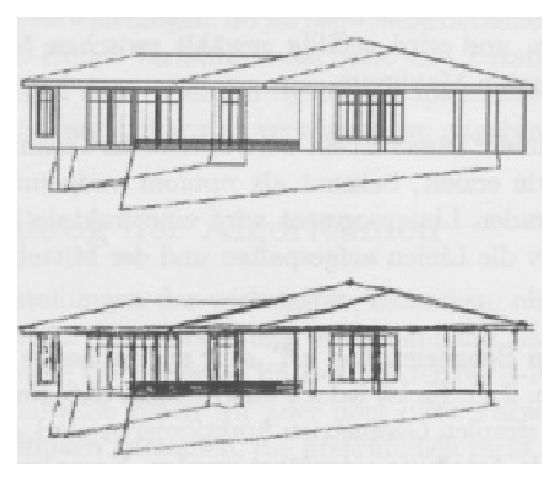
\includegraphics[width=0.60\textwidth]{../images/ComputerSketching}
  \caption{Oben Ausgabe ohne Computer Sketching, unten Ausgabe in der
  "`Sketchy"' Variante}
  \label{fig:ComputerSketching}
\end{figure}

\subsubsection{Noise Modifier}
In einer weiteren Technik im Geometrieraum kommen sogenannte Noise-Modifier zum 
Einsatz, diese erzeugen ein "`Rauschen"' in den 3D-Modellen. Dieses "`Rauschen"' 
wird erreicht, indem die Geometriepunkte der Flächen des Modells um einen 
zufälligen Faktor verschoben werden. Diese Verfahren finden hauptsächlich 
Anwendung auf glatte Flächen, um "`natürliche"' Flächen zu erzeugen.

\subsubsection{Level of Detail}
Ein Verfahren, das in vielen Bereichen Verwendung findet, ist das Level of 
Detail Prinzip, das unterschiedliche Detailstufen zur Darstellung nutzt. Es 
wird unter anderem in der Kartographie eingesetzt. Hier wird die Detailstufe in 
Abhängigkeit vom Maßstab der Karte dargestellt. Ein weiterer Einsatzbereich ist 
die photorealistische Computergrafik. Hier erfolgt die Darstellung der Details 
in Abhängigkeit von der Betrachterposition. Je näher ein Objekt dem Betrachter 
ist, desto genauer wird es dargestellt. NPR modifiziert dieses Prinzip und 
setzt die Detaillevel in Abhängigkeit zur "`Wichtigkeit"' der einzelnen Objekte. 
Je wichtiger ein Objekt für die Darstellung ist, desto genauer wird es 
dargestellt. Eine Möglichkeit zur Umsetzung bietet die Meshsimplifizierung. 
Hierbei wird die Anzahl der Polygone eines "`unwichtigen"' 3D-Modells reduziert 
und die äußere Form approximiert. Diese Technik unterstützt eine schnelle 
Verarbeitung und bietet so einen Einsatz in Echtzeitsystemen.

\subsection{Techniken im Projektionsraum}
Techniken im Projektionsraum werden meist mit Bildraumverfahren kombiniert, um 
ein leichteres Arbeiten mit 3D-Modellen und eine Erhöhung der grafischen 
Qualität der Ausgabe zu ermöglichen. Die Techniken arbeiten nach der Projektion 
und nutzen zusätzliche 3D-Informationen, wie Z-Werte oder Flächennormalen. 
Ein großer Vorteil dieser Techniken ist, wie oben schon angesprochen, die 
leichte Handhabung mit 3D-Modellen und daraus resultierend, die Erhöhung der
grafischen Qualität der Ausgabe. Ein Nachteil ist die komplizierte Berechnung
aufgrund der Verzerrungen. Verfahren, die im Projektionsraum Anwendung finden,
sind G-Buffer, Line-Rendering und Stroke Textures-Verfahren.

\subsubsection{G-Buffer}
Der G-Buffer (Saito u.\ Takahashi, 1990), ausgeschrieben "`Geometrie-Buffer"' 
genannt, ist in den meisten kommerziellen Cartoon-Render-Paketen implementiert. 
Das Prinzip basiert auf einer zusätzlichen Speicherung von geometrischen Daten 
zur Informationsgewinnung im Bildraum. So ist es beispielsweise möglich die 
Flächennormalen, die UV-Koordinaten oder die Z-Buffer-Werte eines 3D-Modells 
zusätzlich zu speichern, dies geschieht im Projektionsraum. Die Informationen 
werden dann für die Bilderzeugung aus dem G-Buffer extrahiert, analysiert und 
zusammengefügt.

\subsubsection{Line-Rendering}
Mit Hilfe der Line-Rendering Methode wird die Semantik von Linien simuliert. 
Dabei wird zwischen geometrischer und stilistischer Semantik unterschieden. 
Unter geometrische Semantik fallen Begrenzungen, Silhouetten, Diskontinuitäten 
und isoparametrische Konturen. Linienstärke, Transparenz und Linientyp 
(gestrichelt, durchgezogen, etc.) hingegen machen die stilistische Semantik 
aus. Im Projektionsraum werden für jede Linie die Charakteristiken, wie 
Wichtigkeit, Linientyp und Verdeckung, zum Beispiel mit Hilfe von 
Inferenzregeln bestimmt. Dann werden diese Attribute in geeigneter Form, etwa 
in Matrixform, abgespeichert und zur Bilderzeugung genutzt. Da sich diese 
Technik primär mit Linienstilen und ihren Semantiken beschäftigt, bietet sie 
eine gute Kombinationsmöglichkeit mit anderen NPR-Techniken, wie etwa mit dem 
zuvor vorgestelltem G-Buffer-Verfahren.

\subsubsection{Stroke Textures}
Das Prinzip der Stroke Textures (Winkenbach \& Salesin, 1994) basiert auf 
konventionellen 2D-Malsystemen. Es wird eine "`strichbasierte"' Textur 
angefertigt, die mittels Texturemapping auf bereits projizierte 3D-Objekte 
aufgebracht wird. Hierbei ist eine Anwendung des LOD-Prinzips auf die Textur 
möglich. Der Benutzer ist in der Lage die Linienstärke sowie sogenannte 
"`Detail Tags"' zu spezifizieren, um eine genauere Darstellung der Textur an 
ausgewählten Stellen zu erreichen.

\subsection{Techniken im Bildraum}
Bei Techniken im Bildraum geht man von einem vorhandenen Bild aus, das 
analysiert und neu "`gezeichnet"' wird. Vorteilhaft ist hierbei, dass das Bild 
bereits vorhanden ist, also keine Viewing-Pipeline nötig ist. Ein tragender 
Nachteil der Verfahren ist der, dass im Bildraum nur ungenauere Berechnungen 
möglich sind. Einige Verfahren, die im Bildraum angewendet werden, sind Texture 
Elements, Hairy Brushes und das Iterated Funktion System.

\subsubsection{Texture Elements}
Textur Elements (Mezei et al\., 1974) wurden ursprünglich zur Synthese sehr 
"`naturalistischer"' Bilder eingesetzt, da man in Beobachtungen festgestellt 
hatte, dass in der Natur sich wiederholende Muster vorkommen. Hierbei werden 
grafische Subelemente (größer als ein Pixel), die sogenannten "`Texture 
Elements"', vorgefertigt. Diese Elemente werden dann im eigentlichen 
Bilderzeugungsprozess zusammengefügt und ergeben so das neue Bild. Um 
Variationen im Bild zu erreichen, werden Skalierungen, Rotationen und andere 
Verzerrungen auf die Texture Elements angewendet. So werden Verallgemeinerungen 
der Oberflächeneigenschaften erzielt, die wie menschliche Illustrationen wirken.

\subsubsection{Hairy Brushes}
Mit dem Verfahren Hairy Brushes versuchte Strassmann 1986 als einer der ersten 
das Verhalten von Pinsel und Farbe zu simulieren. Der Pinsel wird dabei als 
1D-Abdruck seiner Borsten implementiert. Diese Borsten laufen an einer 
parametrisierten Kurve entlang, die durch Knoten definiert ist. Jeder dieser 
Knoten enthält Informationen über Position und Druck des Pinsels. Der Druck 
wird zwischen den Knoten interpoliert und gibt an, wie viel Farbe der Pinsel an 
den Zeichenuntergrund abgibt. Jeder "`Strich"' wird mit einer speziellen Menge 
an Farbe gezeichnet, die mit zunehmender Länge des "`Striches"' abnimmt. Die 
Farbe kann durch ein "`Eintunken"' des Pinsels wieder aufgefüllt werden, dies 
ermöglicht auch Variationen in der Farbe.

\subsubsection{Iterated Function System (IFS)}
Iterated Function System beschreibt ein System von Funktionen die wiederholt 
ausgeführt werden. Das System wird vor allem zur Beschreibung von Fraktalen 
eingesetzt. Fraktale sind selbstähnlich, d.\,h\. sie sind rekursiv aufgebaut. 
Eines der bekanntesten Beispiele ist der Barnsley-Farn. Der Rekursive Aufbau 
ist besonders gut in den Farnblättern zu erkennen (siehe Abbildung 
\ref{fig:BarnsleyFarn} und Abbildung \ref{fig:BarnsleyFarnDetail}).

\begin{figure}
  \centering
  \subfloat[Barnsley Farn]{
    
\includegraphics[width=0.3\textwidth]{../images/BarnsleyFarn.eps}
    \label{fig:BarnsleyFarn}
  }
  \qquad
  \subfloat[Barnsley Farn Detailansicht]{
    
\includegraphics[width=0.3\textwidth]{../images/BarnsleyFarnDetail.eps}
    \label{fig:BarnsleyFarnDetail}
  }
\end{figure}

Barnsley nutzte das Prinzip des IFS 1988 zur fraktalen Kompression von Bildern. 
Diese Kompressionstechnik basiert auf der Selbstähnlichkeit von Bildern, dem 
sogenannten "`Collage Theorem"'. Zwischen größeren und kleineren Teilen eines 
Bildes lassen sich bestimmte Ähnlichkeiten finden. Das zu komprimierende Bild 
(\ref{fig:IFS_Lena}) wird hierbei in "`range blocks"' unterteilt, dabei ist 
eine gleichmäßige Aufteilung möglich, wobei jeder Block im Allgemeinen eine 
Größe von 8x8 Pixeln besitzt. Aber auch eine Quadtree-Unterteilung ist denkbar, 
um Details besser wiedergeben zu können. (siehe Abbildung \ref{fig:Quadtree_Lena})

\begin{figure}
  \centering
  \subfloat[Lena]{
    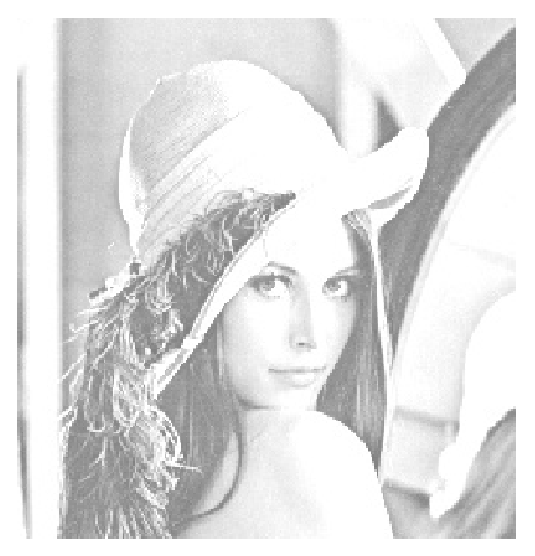
\includegraphics[width=0.4\textwidth]{../images/IFS_Lena.eps}
    \label{fig:IFS_Lena}
  }
  \qquad
  \subfloat[Quadtree-Unterteilung]{
    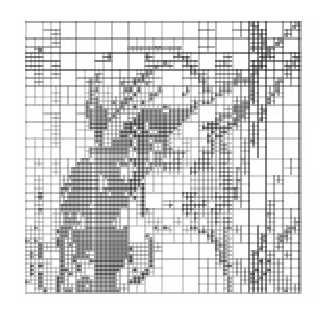
\includegraphics[width=0.45\textwidth]{../images/Quadtree_Lena.eps}
    \label{fig:Quadtree_Lena}
  }
\end{figure}

%%% Inkludieren Kapitel 3
\chapter{Einsatzgebiete}
\section{Anwendungen}
Die Anwendung des NPR ist vielfältig: Strichzeichnungen sind im Bereich 
technischer Anleitungen oft besser verständlich als Fotos, auch in 
medizinischen Fachbüchern bilden Fotos eher eine Ausnahme. \par In anderen 
Bereichen, in denen es bisher üblich war, Zeichnungen von Hand anzufertigen, 
werden heute CAD- Programme eingesetzt. Um hierbei die selben Ergebnisse wie 
früher zu erreichen, ist oft ebenfalls NPR nötig (als Beispiel sei die 
Zeichnung von Architekten genannt, bei der der Detailgrad einer Strichzeichnung 
den Stand der Planung widerspiegelt). Ferner spielt NPR im künstlerischen 
Bereich und in Computerspielen eine große Rolle.

\subsection{Zeichentrickfilme}
Zeichentrickfilme oder Cartoons, kurze Filme die aus einer Aneinanderreihung 
von, zumeist handgezeichneten, Einzelbildern entstehen, werden heutzutage meist 
mit dem Computer produziert. Dabei werden 3D-Programme verwendet, die mit Hilfe 
eines Toon-Shaders die animierten Figuren so aussehen lassen, als seien sie von 
Hand gezeichnet. The Walt Disney Company, einer der größten Produzenten von 
Zeichentrickfilmen beschäftigt mittlerweile keinen einzigen Zeichner mehr, 
sondern setzt vollkommen auf die Computeranimation. Dabei wird vor allem der 
verringerte Aufwand sowie die schnellere Produktion und die geringeren Kosten 
gegenüber der handgezeichneten Variante als Vorteil genannt. Aber auch 
einfachere Umschnitte und Gegenperspektiven sowie Schwenks durch die Szenerie 
sind ein Vorteil der computerunterstützen Animation. Toon-Shader kommen meist 
nach dem Rendern zum Einsatz, in dem sie zunächst die Farbtiefe auf einige 
Zwischentöne reduzieren. Um schwarze Außenlinien zu produzieren, werden bei 
der Darstellung die Polygone einfach umgedreht und die schwarze Rückseite 
gezeichnet, meist mehrfach und leicht verschoben. Anschließend werden die 
Polygone wieder korrekt gezeichnet um Farbverläufe und optional auch Texturen 
darzustellen. Wird das Bild nun über den Z-Buffer zusammengesetzt, erscheinen 
die umgedrehten Polygone, welche immer tiefer sind als die anderen, als 
schwarze Konturen um die Objekte.

\subsection{Architektur}
Architekten verwenden gerne vereinfachende Verfahren der nicht-realistischen 
Computergraphik. Zu detailreiche Ansichten von Häusern oder anderen 
geometrischen Figuren überfordern den Kunden meist und werfen viele Fragen auf. 
Um diesem Problem zu begegnen verwenden Architekten oftmals einen reduzierten 
Bauplan und versuchen die Darstellung so weit zu abstrahieren, dass der Kunde 
gezwungen ist, die eigene Vorstellungskraft einzusetzen. Dies ist oft sehr 
hilfreich, da gerade die einfach gezeichneten Pläne leichter aufzunehmen sind 
und das Gehirn kann die Vorstellung besser in die reale Welt integrieren, als 
zu perfekt animierte Häuser, die den Eindruck erwecken, bereits gebaut worden 
zu sein. Vereinfachte Animationen helfen den Bauherren hingegen ihre 
Kreativität zu aktivieren und Raum für Veränderungen und Visionen zu geben.

\subsection{Maschinenbau}
Im Maschinenbau müssen oftmals Prinzipien die in komplexe Maschinen verpackt 
sind anschaulich erläutert werden. Ob in Bauplänen und Bedienungsanleitungen, 
oder in Forschungsberichten, die neuartige Prinzipien und deren Umsetzungen 
verdeutlichen sollen, es bleibt das Problem, dass vereinfachte Darstellungen 
von Modellen und Prinzipien verdeutlicht werden müssen. Da die reinen 
CAD-Zeichnungen absolut vollständig sind, ist es relativ schwer in ihnen die 
wichtigen Informationen zu erkennen. Um das unwichtige wegzulassen, generiert 
man hieraus gerne Explosions- oder Schnittzeichnungen (s.\ Abbildung 
\ref{fig:explosion}), die nur die wesentlichen Bestandteile zeigen. Andere 
Fälle sind beispielsweise halbtransparente Darstellungen von Automobilen, bei 
denen die Komponenten des Bremssystems hervorgehoben sind. Dies vereinfacht die 
Aufnahme in dem die Informationen auf das Wesentliche reduziert werden. In 
Bedienungsanleitungen wird auch gerne die Maschine als ganzes vereinfacht 
dargestellt, so dass man letztlich nur noch die Oberfläche der Mikrowelle 
darstellt, da dies absolut ausreichend ist, um ihre Bedienung zu erläutern.

\begin{figure}
  \centering
  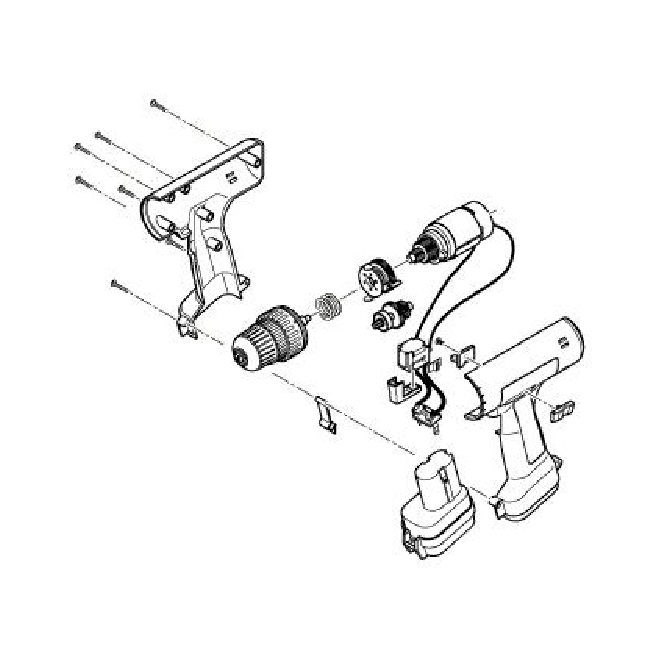
\includegraphics[width=0.5\textwidth]{../images/explosion}
  \caption{Beispiel für eine Explosionszeichnung}
  \label{fig:explosion}
\end{figure}

\subsection{Medizin}
Ebenso ist in der Medizin beispielsweise der Blutkreislauf oder ähnliches nicht 
einfach durch Fotos eines aufgeschnittenen Körpers darzustellen. Auch ein 
fotografiertes Herz enthält zu viele Details um als lehrreiche Skizze zu dienen.
 Generell kann man also der nichtrealistischen Computergraphik davon ausgehen, 
dass es sich um eine Designentscheidung handelt, die dem ungeübten Auge den 
Zugang zu Informationen durch Weglassung erleichtert.

\subsection{Biologie}
Ebenfalls ist in der Biologie weit verbreitet, Arten durch Skizzen einer 
Pflanze darzustellen. Diese beispielhaften Exemplare sind so in der Natur meist 
niemals zu finden, da sie in idealer Weise alle Merkmale in sich vereinen ohne 
zu viele Informationen darzustellen und so den Biologen zu verwirren. Es handelt
 sich also auch in diesem Fall um eine Unterstützung des Menschen durch 
Generalisierung der Merkmale einer Klasse von Pflanzen oder Tieren, die somit 
leichter wieder erkannt werden können. Zeichnete man diese Vorzeigekandidaten 
früher noch von Hand, übernimmt diese Arbeit nun oftmals der Computer. Es wäre 
einfach, eine realistische Pflanze zu erstellen die wie auf einem Foto 
aussieht. Die schwierigere Variante ist, die wichtigen Informationen 
herauszudestillieren und es so aussehen zu lassen, als wäre es eben diese 
abstrakte Repräsentation der Klasse von Pflanzen, um so dem Biologen die 
Möglichkeit der Klassifikation zu geben.

\subsection{Kartographie}
In der Kartographie versucht man ebenfalls viele Informationen auf einem 
kleinen Raum schematisch abstrahiert darzustellen. So finden sich 
beispielsweise Informationen über den Boden, das Klima, die Pflanzenwelt und 
Höheninformationen in der jeweiligen Farbzeichnung des Ausschnitts wieder. 
Erkennt man dies auf detailreichen Satellitenbildern ebenso gut? Sicherlich 
wäre ein Fachmann ohne Probleme dazu in der Lage, doch die vielen detailreichen 
Informationen würden einen Laien nur verwirren, könnte er sie überhaupt 
erkennen. Es muss also wieder zusammengefasst und abstrahiert werden, um die 
Informationen leicht zugänglich zu machen. Dieser Prozess ist keinesfalls 
einfach und darum kommen hier auch keine automatisierten Verfahren zum Einsatz, 
obwohl dies technisch durchaus möglich wäre. Aber um den Detailgrad richtig zu 
wählen und die Informationen präzise zu setzen muss ein Fachmann die 
Informationen filtern und viele Quellen zu einer einzigen Karte zu Rate ziehen. 
Diese Informationen werden nun zusammengeführt und schlagen sich beispielsweise 
in der Farbe der Erde an der jeweiligen Stelle nieder. Es kann durchaus sein, 
dass auf einer Karte der Alpen Schnee eingezeichnet ist, obwohl auf den 
Satellitenbildern der letzten 3 Jahre dort nachweislich kein Schnee gelegen 
hat. Aber über die Höhe und die Gegebenheiten ist nunmal entschieden worden, 
dass es eben generell möglich wäre, dass an dieser Stelle beispielsweise ein 
Gletscher entstehen kann. Ein weiteres Szenario ist die Simulation von 
Hochwasser und so die Möglichkeit hochwassergefährdete Gebiete einzuzeichnen 
obwohl hier eventuell noch nie ein Hochwasser in dieser Gegend war. Durch 
Physiksimulation der Landschaft sind diese Karten für die Bebauungsplanung aber 
ein wertvoller Hinweis, und sie können leicht von den zuständigen Behörden 
interpretiert werden, da die Informationen leicht zugänglich in der Karte über 
nicht-realistische Computergraphik dargestellt werden kann.

%%% Inkludieren Kapitel 4 (Schwerpunkt)
\chapter{Synthetische Pflanzenskizzen}
\section{Einführung}
Um solche synthetischen Pflanzenskizzen zu erzeugen, bedient man sich der 
Schraffurtechnik. Durch diese Technik erhält man ein hohes Maß an 
Detailreichtum, Anwendung neben der Erzeugung solcher synthetischer 
Pflanzenskizzen ist auch die Erzeugung synthetischer Kupferstiche, was eine 
seit dem Mittelalter genutzte Technik ist.
\par Grundsätzlich hängt eine solche Schraffur von einigen Parameter an:

\begin{itemize}
  \item von Schatten und Helligkeitsabstufungen im Originalbild
  \item von Objekt- und Materialeigenschaften (Kanten, Falten; Texturen)
  \item von Unterschiedlichen Farben
\end{itemize}

Eine weitere Frage, die man sich stellt ist "`Wie kann man Schraffuren 
variieren?"'

\begin{itemize}
  \item Wo sind Linien?
  \item Länge der Linien
  \item Wie verlaufen sie? In Bezug auf Richtung und Linienart
  \item Parallelität der Linien innerhalb einer Schraffur
  \item Dichte der Linien
\end{itemize}

Das Einsatzgebiet solcher Schraffuren ist vielfältig, man findet diese in 
Bleistiftzeichnungen, bei Linien im NPR-Bereich: detailreiche Karikaturen, 
Bewegungslinien in Cartoons, in Stroke-based Illustrations, bei der Simulation 
von Holzschnitten, Kupferstichen oder eben bei Pflanzenskizzen.

\section{Funktionsweise}
Zuerst wollen wir hier auf die Erzeugung solcher Schraffuren bei synthetischen 
Kupferstichen eingehen, da die Technik grundlegend ist, um auch synthetische 
Pflanzenskizzen erzeugen zu können. Der algorithmische Ansatz zur Herstellung 
solcher Schraffuren interpretiert die Schraffurlinien als Schnitte zwischen der 
darzustellenden dreidimensionalen Geometrie und einer Schar von Ebenen. Andere 
Verfahren verwenden Volumenfunktionen oder Hauptkrümmungsrichtungen. \par Die 
Verwendung von Schnittebenen hat den Vorteil, dass man die Ebenenschar auf eine 
Weise spezifizieren kann, die den Linien ästhetisch ansprechende Formen 
verleihen.
Zusammenfassend lässt sich das Verfahren also wie folgt strukturieren:

\begin{itemize}
  \item Zerlegung des Geometriemodells in einzeln zu schraffierende Teile
  \item pro Teil: Spezifikation einer Ebenenschar mittels graphischem Editor
  \item Berechnung der Schnittlinien der Ebenen
\end{itemize}

Dadurch soll die Form der Schraffurlinien wiedergegeben werden (wie Geometrie, 
Lichtverhältnisse $\to$ Liniendicke). \par Das Ziel bei der Herstellung 
synthetischer Pflanzenskizzen ist die Vermittlung des Eindrucks eines Modells 
einer Landschaft durch Form und Größenverhältnisse, ohne eine konkrete 
Ausprägung zu erreichen. Um beispielsweise eine Baumskizze zu erzeugen, muss 
dieser durch 2 Arten von Geometrie beschrieben werden:

\begin{itemize}
  \item Astwerk mit glatter Oberfläche
  \item Blattwerk aus vielen tausend Einzelflächen
\end{itemize}

Das heißt konkret, dass hier zwei separate Algorithmen zum Einsatz kommen 
müssen, um die Strukturunterschiede erzeugen zu können. Zur Darstellung des 
Baumstamms wird eine ähnliche Technik wie bei Kupferstichen verwendet: Es wird 
die Silhouette gezeichnet und Schraffurstriche an den Stellen, die wenig 
beleuchtet sind. Hierfür wird eine Variante der Halftoning-Methode eingesetzt, 
die diesmal aber keine Punkte, sondern kurze Striche erzeugt. In nachfolgender 
Abbildung \ref{fig:Baum} ist ein Beispiel zu sehen.

\begin{figure}
  \centering
  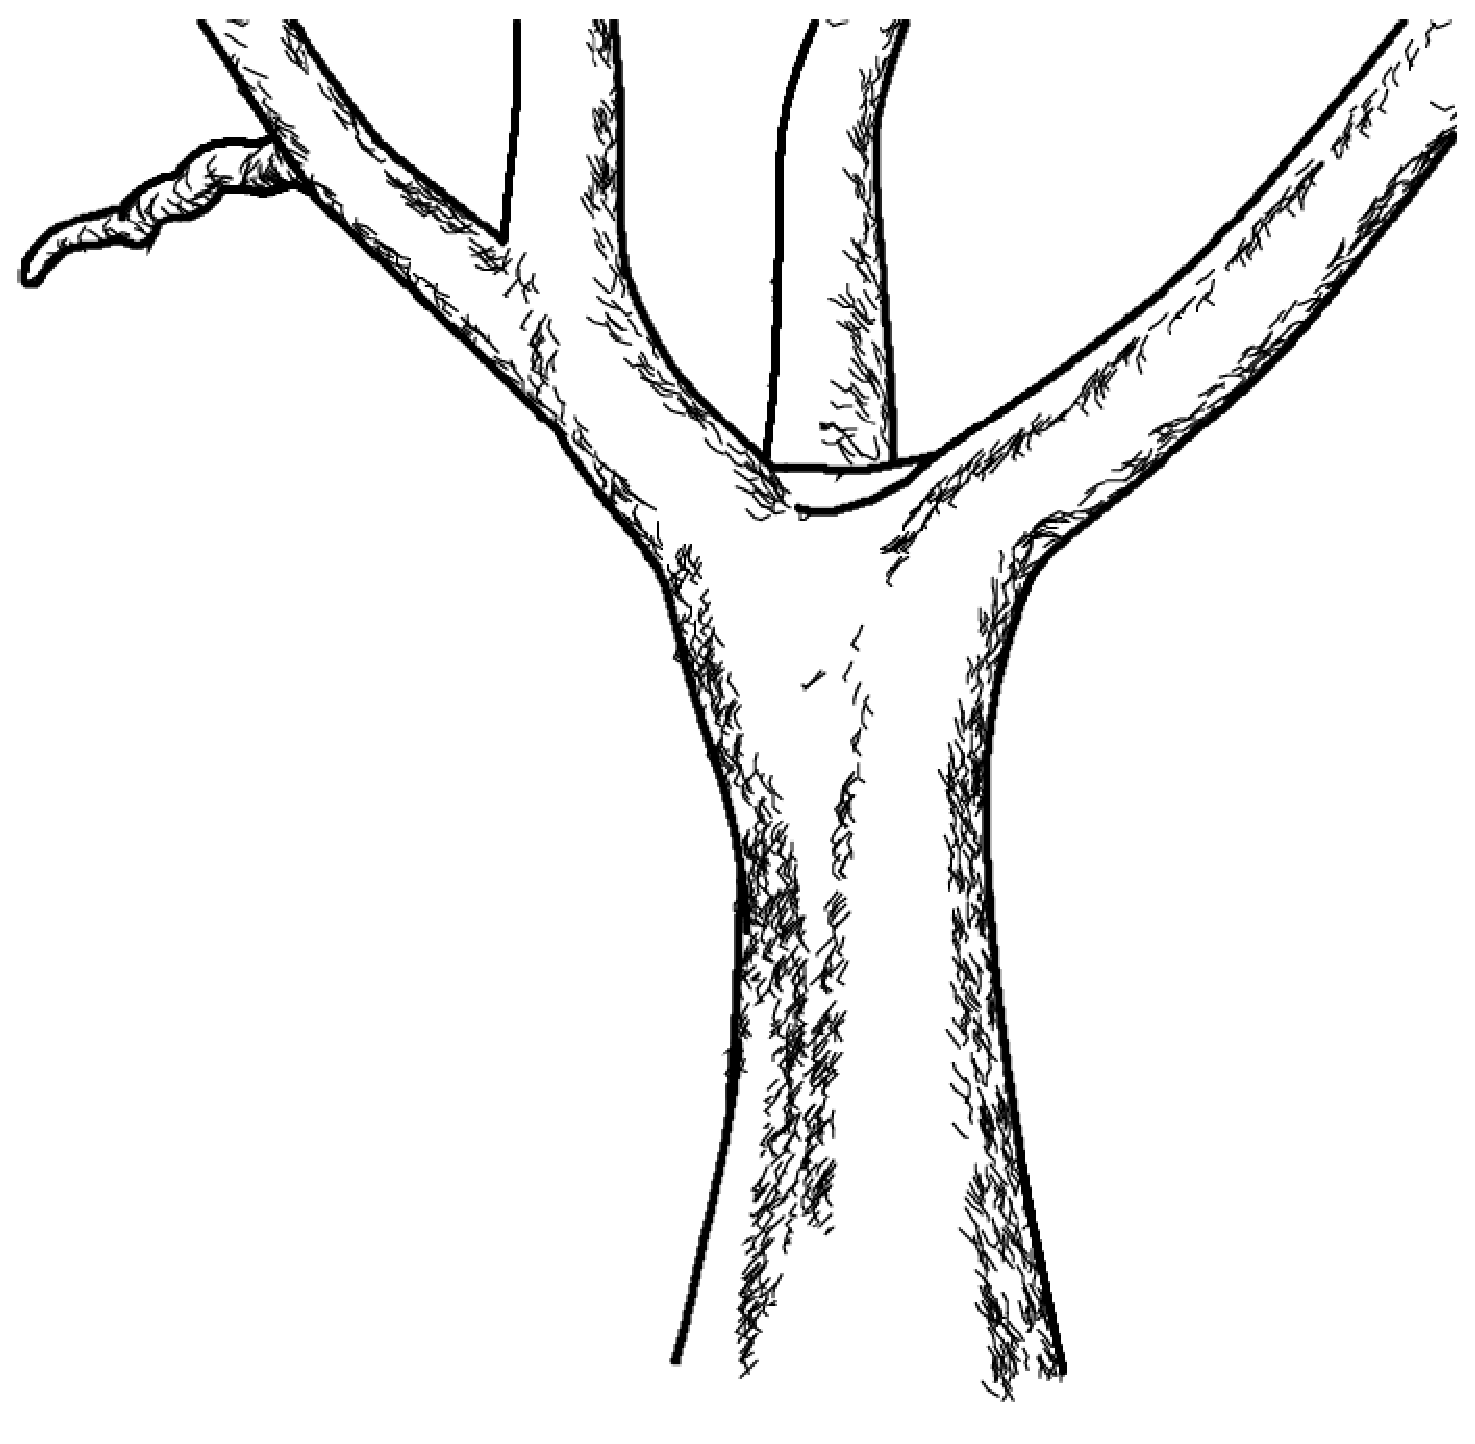
\includegraphics[height=6cm]{../images/Deussen2000-tree-trunk-branches}
  \caption{Stamm und Hauptäste von Baum 1. Quelle: \cite{Deussen2000}.}
  \label{fig:Baum}
\end{figure}

\section{Beispielgrafiken für erzeugte Baumskizzen}
Abschließend sind hier ein paar weitere Beispiele für synthetische Baumskizzen
aufgeführt. Abbildung \ref{fig:baum1-varianten} zeigt dabei den bereits
vorgestellten Baum 1 inkl.\ Blattwerk.

\begin{figure}
  \centering
  \subfloat{
    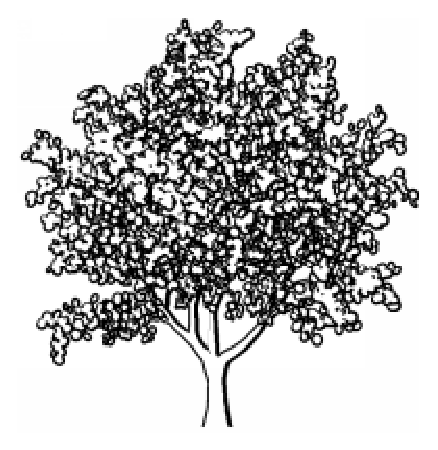
\includegraphics[height=6cm]{../images/Deussen2000-tree1-version1}
  }
  \qquad
  \subfloat{
    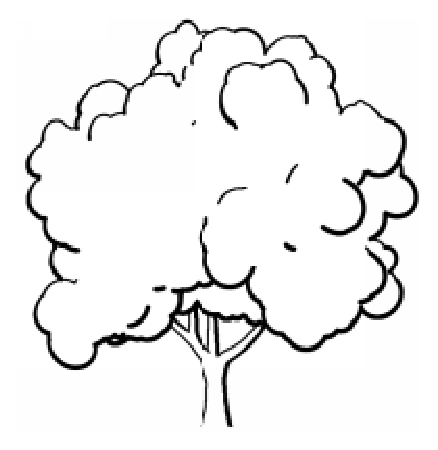
\includegraphics[height=6cm]{../images/Deussen2000-tree1-version2}
  }
  \caption{Baum 1 mit verschiedenen Parametern für Blattwerk und Detailgrad.
  Quelle: \cite{Deussen2000}.}
  \label{fig:baum1-varianten}
\end{figure}

Neben einzelnen Bäumen lässt sich zusätzlich auch die direkte Umgebung eines
Baumes darstellen, wie Abbildung \ref{fig:baum-gross} zeigt.

\begin{figure}
  \centering
  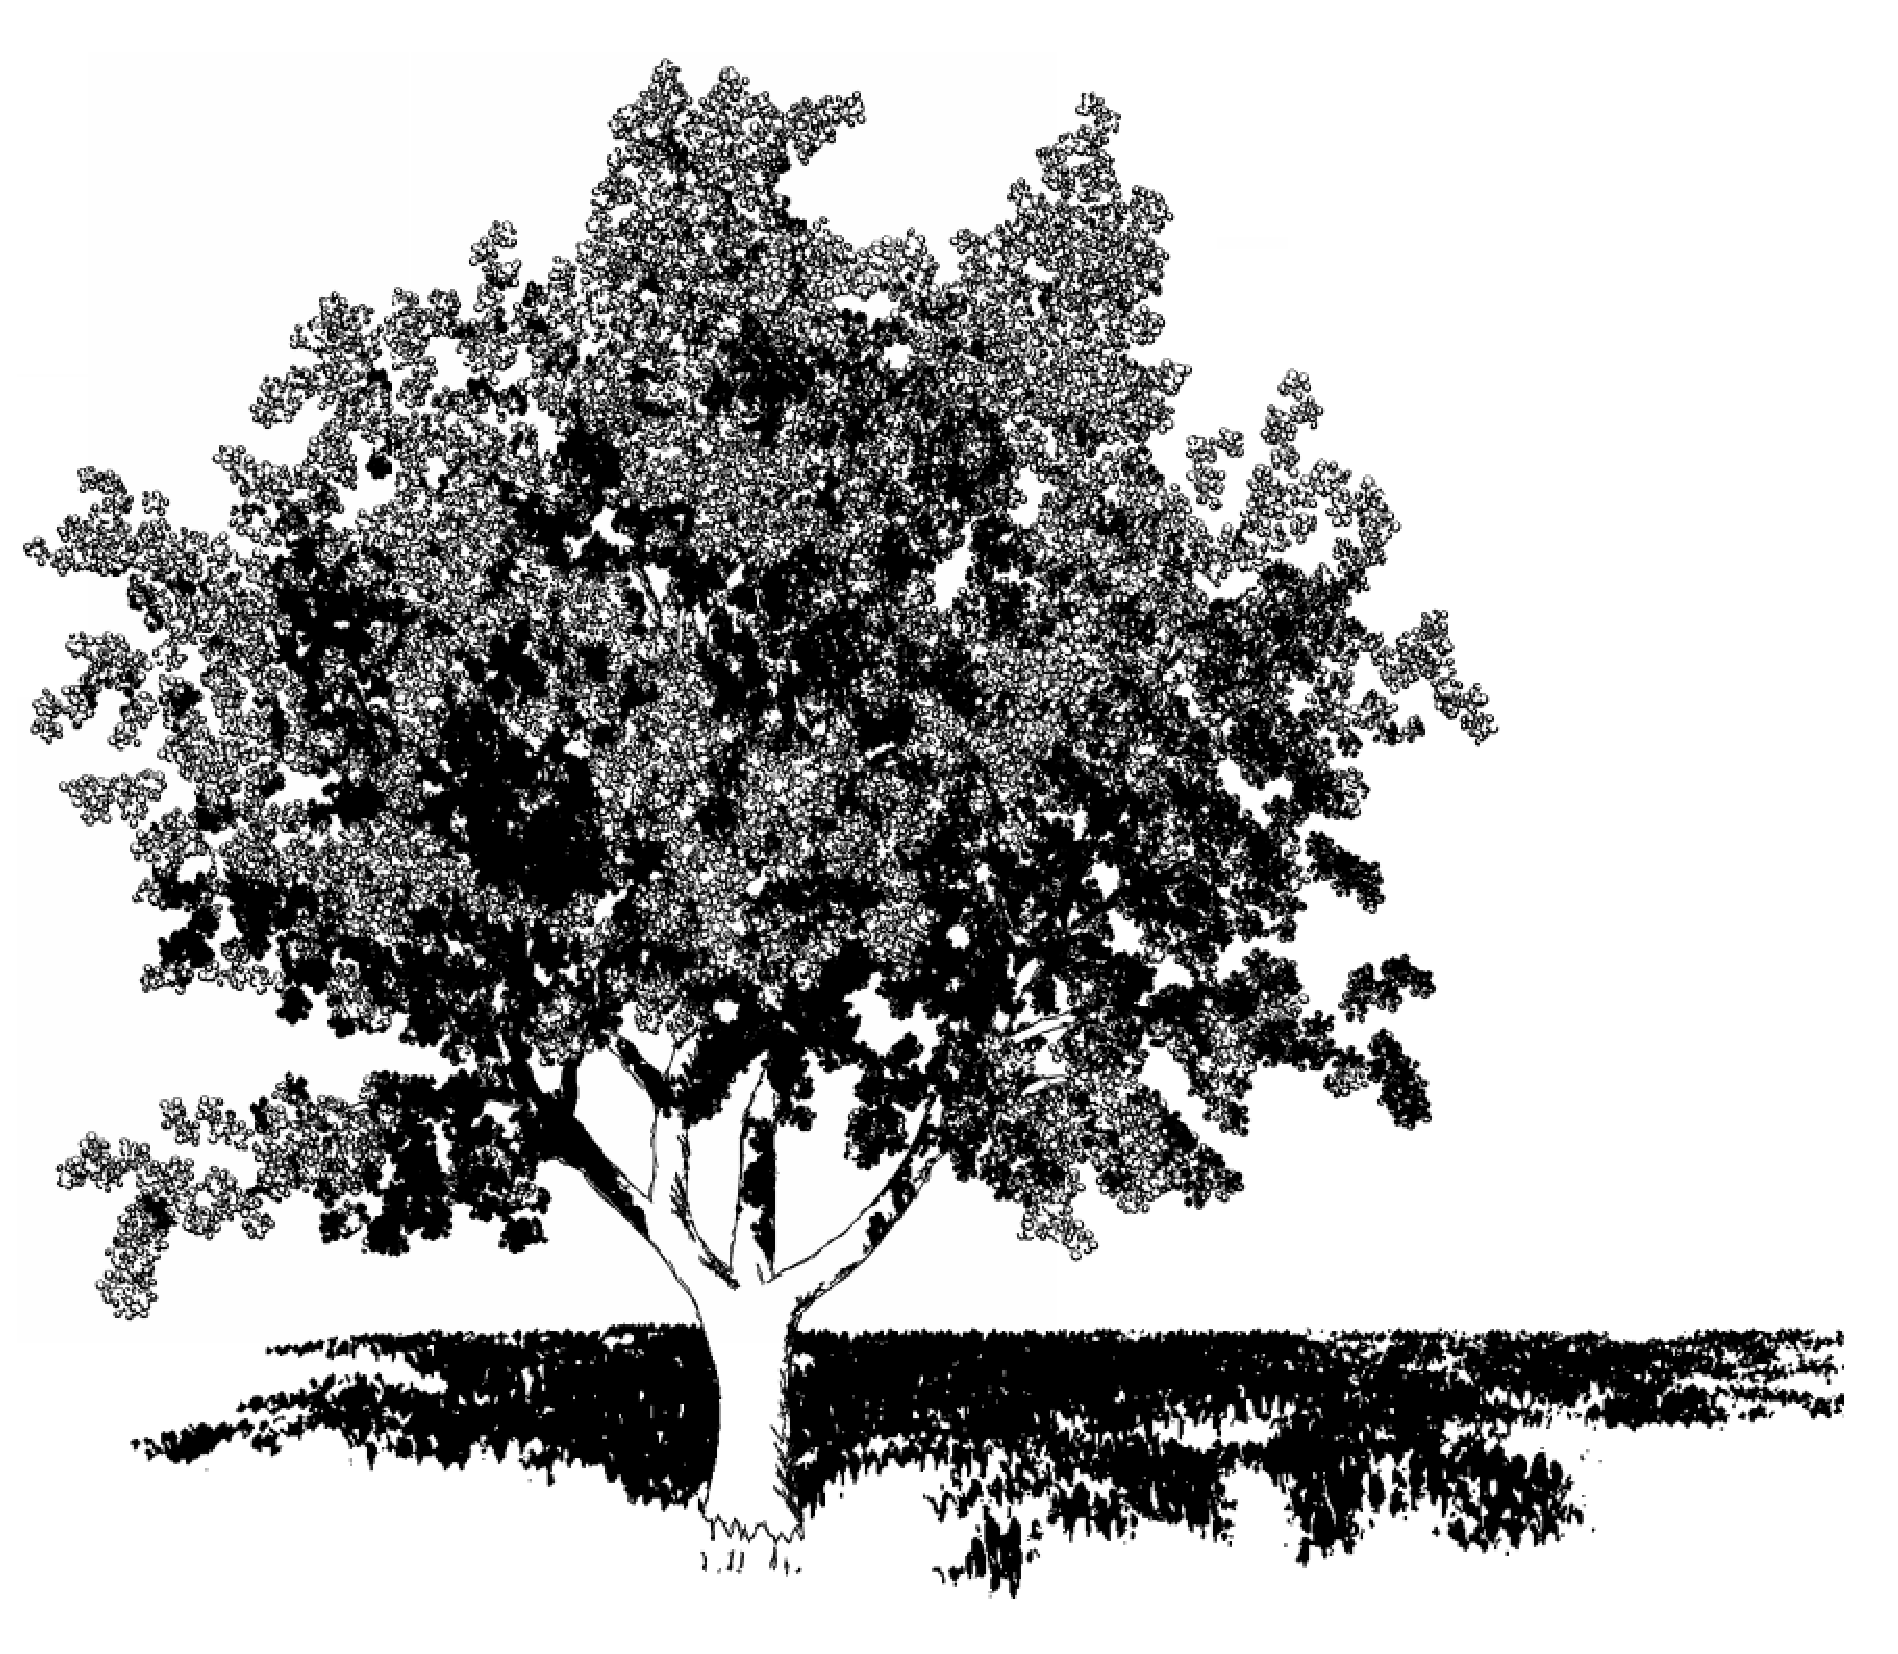
\includegraphics[width=0.8\textwidth]{../images/Deussen2000-tree-large}
  \caption{Baum 3 mit Grasumgebung. Quelle: \cite{Deussen2000}.}
  \label{fig:baum-gross}
\end{figure}

%%% Inkludieren Kapitel 5 (Schwerpunkt)
\chapter{Wasserfarbenillustration}
\section{Einführung Wasserfarben}
Die moderne Form der Malerei mit Wasserfarben erlangte Ende des 18.\ 
Jahrhunderts ihre breite Anerkennung. Mithilfe von Wasserfarben lassen sich die 
unterschiedlichsten Effekte und Strukturen erzielen, die beispielsweise durch 
das Wandern der im Wasser gelösten Farbpigmente über das Papier entstehen. In 
den nächsten Abschnitten sollen die grundlegenden hierzu verwendeten 
Materialien und Techniken kurz vorgestellt werden.

\subsection{Materialien}
Das bei der Wasserfarbenmalerei verwendete \textbf{Papier} ist zumeist nicht 
wie üblich aus Zellstoff (also z.\,B.\ Baumholz), sondern aus Leinen oder 
Baumwolle hergestellt. Das Papier erhält durch die netzartige Struktur sein 
charakteristisches, unebenes Erscheinungsbild. Zur Imprägnierung des Papiers 
wird Zellulose benutzt, welche die Fasern umhüllt und einige der Poren 
ausfüllt. Auf diese Weise kann Wasser nicht mehr völlig ungehindert absorbiert 
werden - die Struktur bleibt trotzdem erhalten.

Die eigentliche \textbf{Wasserfarbe} besteht aus in Wasser gelösten Pigmenten,
einem Bindemittel sowie einem Tensid (oberflächenaktiver Stoff). Pigmente
bestehen aus einzelnen festen Partikeln und werden typischerweise zu einem Puder
verarbeitet. Sie können in das Papier eindringen und sich mithilfe des
Bindemittels anhaften. Pigmente unterscheiden sich in ihrer Dichte - eine hohe
Dichte sorgt dafür, dass sich das Pigment im Wasser nicht sehr weit bewegen
kann, bei geringer Dichte können die Partikel weiter "`wandern"'.
Das Tensid dient dazu, die Oberflächenspannung des Papiers herabzusetzen und es
dem Wasser so zu ermöglichen, in das Papier einzudringen und es zu durchtränken.

\subsection{Techniken}
Es werden hauptsächlich zwei Pinseltechniken verwendet. Zum einen das sog.\ 
\textsl{wet-on-wet}-, zum anderen das \textsl{wet-on-dry}-painting. Bei der
ersten Maltechnik wird mit einem nassen und farbgetränkten Pinsel auf bereits
nassem Papier gemalt. Auf diese Weise kann sich das Wasser und somit die Farbe
frei verteilen. Beim \textsl{wet-on-dry}-painting hingegen wird auf trockenem
Papier gemalt. Beide Techniken erzeugen die für die Wasserfarbenmalerei
charakteristische Effekte, welche im nächsten Abschnitt vorgestellt werden
sollen.

\subsection{Effekte}
Durch das Zusammenspiel von Wasserverlauf, Papierstruktur und Pigmentdichte 
können bei der Wasserfarbenmalerei die verschiedensten Effekte erzielt werden. 
In Abbildung \ref{fig:effects-real} sind die wichtigsten dieser Effekte 
aufgeführt.

\begin{figure}
  \centering
  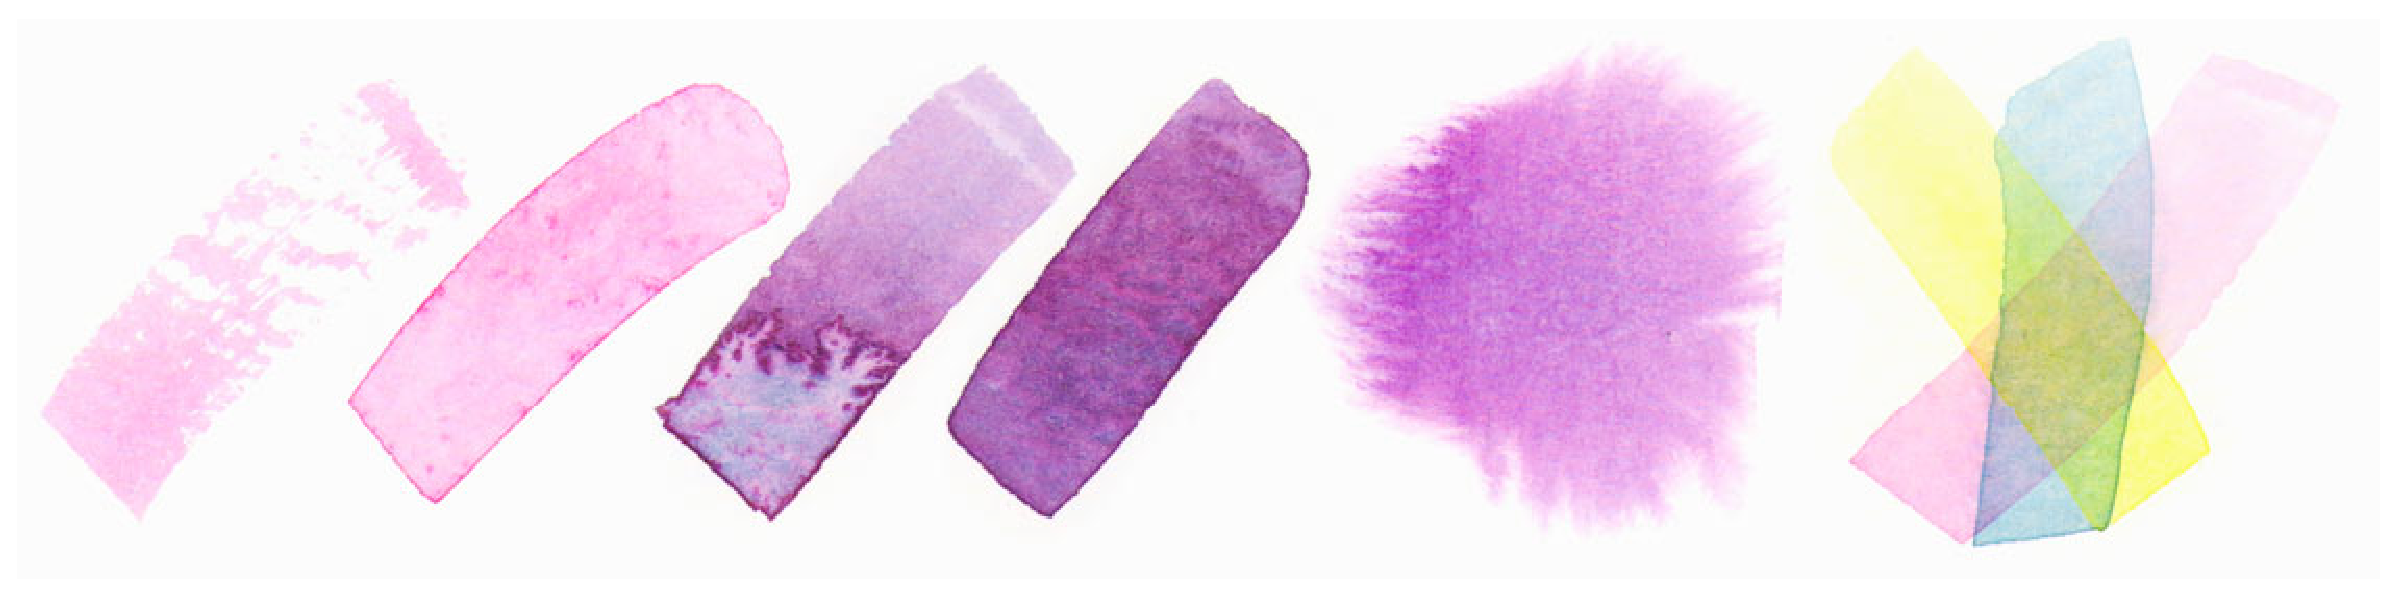
\includegraphics[width=1.00\textwidth]{../images/Curtis1997-real-watercolor-effects.eps}
  \caption{Wasserfarbeneffekte v.l.n.r.: drybrush, edge darkening, backrun,
  granulation, flow effect, glazing. Quelle: \cite{Curtis1997}.}
  \label{fig:effects-real}
\end{figure}

Bei der Verwendung der \textsl{wet-on-wet}-Pinseltechnik können die folgenden
Effekte entstehen:

\begin{itemize}
  \item \textsl{backrun}: Tritt auf, wenn eine Wasserlache zurück in eine
  feuchte Region fließt und das Wasser auf diese Weise Pigmente weiter verteilt.
  Es entstehen komplexe, verzweigte Formen mit teilweise dunklen Kanten.
  \item \textsl{ganulation}, \textsl{separation}: Die Granulierung der Pigmente
  ergibt eine körnige Textur, welche die Spitzen und Täler des Papiers betont.
  Je nach Pigment fällt die Granulierung natürlich anders aus und der Effekt
  kommt am stärksten bei sehr nassem Papier zum tragen. \textsl{Separation}
  bedeutet, dass unterschiedlich dichten Pigmente verschieden weit transportiert
  werden und somit eine Trennung der Farben entsteht.
  \item \textsl{flow pattern}: Die nasse Oberfläche des Papiers ermöglicht, dass
  der Pinselstrich sich frei ausbreitet und weiche, federartige Formen erzeugt
  werden. 
\end{itemize}

Die folgenden Effekte werden mithilfe der \textsl{wet-on-dry}-Technik erzeugt:

\begin{itemize}
  \item \textsl{dry brush}: Wird der trockene Pinsel im richtigen Winkel
  angewandt, so werden nur die erhabenen Stellen des Papiers mit Farbe bedeckt.
  Darus entstehen unregelmäßige Lücken mit ausgefransten Kanten.
  \item \textsl{edge darkening}: Während des Trockenvorgangs wandern die 
  Pigmente aus dem inneren des Pinselstrichs nach außen. Auf diese Weise 
  entstehen dunkle Schattierungen an den Kanten.
  \item \textsl{glazing}: Werden mehrere, dünne Farbschichten nach dem Trocknen
  übereinander gemalt, sodass die einzelnen Farbschichten optisch gemischt werden.
\end{itemize}

\section{Computer-erzeugte Wasserfarben}
Bei der Simulation von Wasserfarben kommt es nach \cite{Curtis1997} darauf an, 
nicht nur die physikalischen Eigenschaften des Mediums zu berücksichtigen, 
sondern auch die für diese Maltechnik charakteristischen Phänomene - nur wenn 
diese realistisch wiedergegeben werden können, ist die Simulation gelungen.

\subsection{Simulation}
In den folgenden Kapiteln wird die Simulation von Wasserfarben nach
\cite{Curtis1997} mit ihren einzelnen Teilbereichen näher beschrieben. Abbildung
\ref{fig:effects-simulated} zeigt die Ergebnisse der Simulation anhand der
bereits vorgestellten Effekte.

\begin{figure}
  \centering
  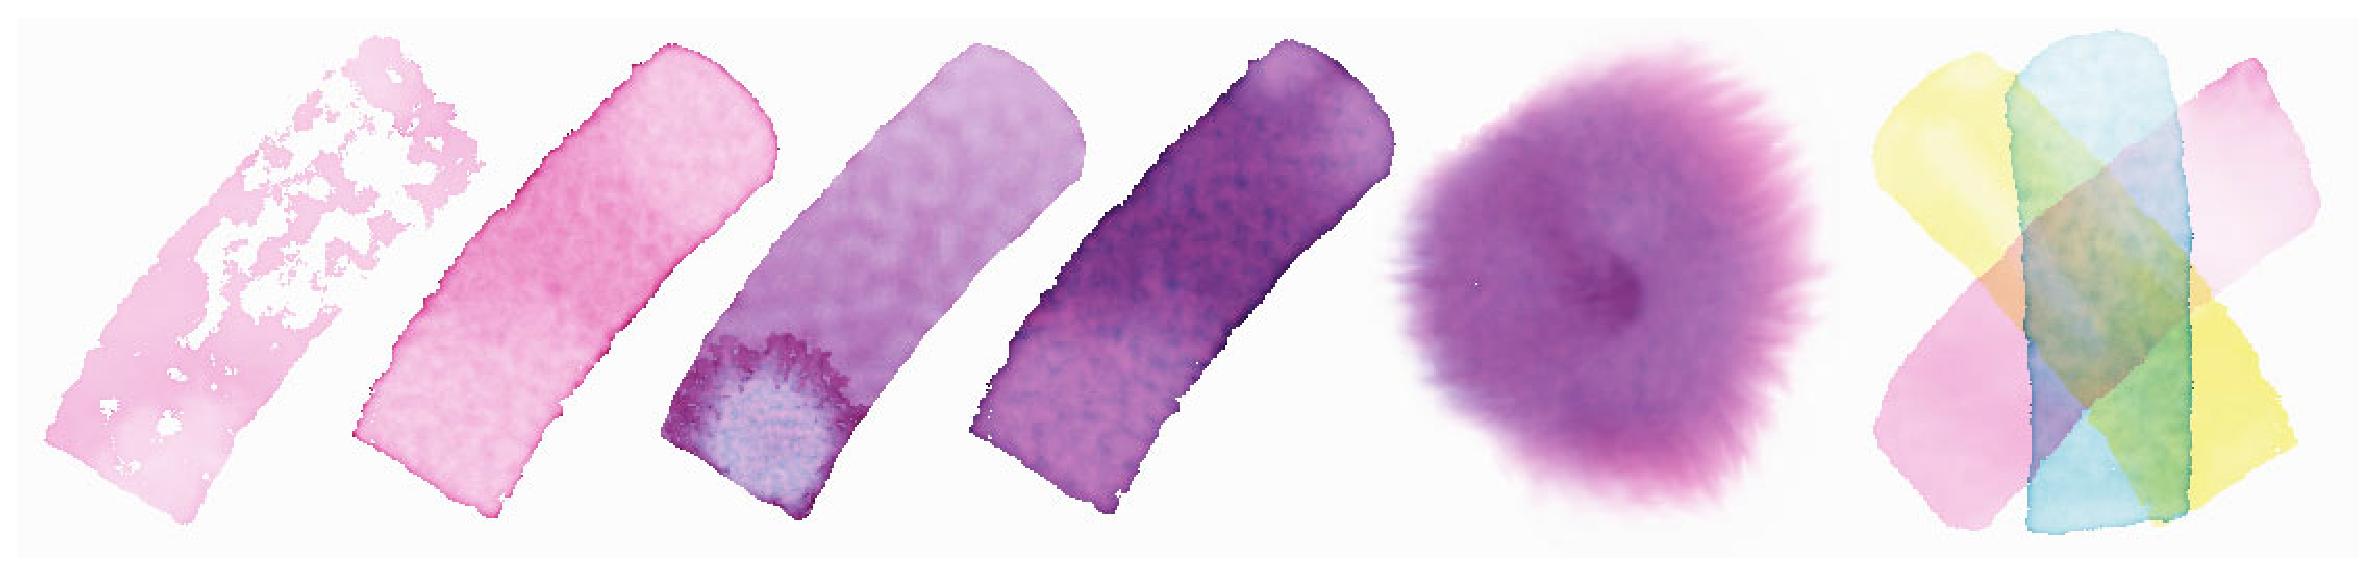
\includegraphics[width=1.00\textwidth]{../images/Curtis1997-simulated-watercolor-effects.eps}
  \caption{Simulierte Wasserfarbeneffekte. Quelle: \cite{Curtis1997}.}
  \label{fig:effects-simulated}
\end{figure}

\subsubsection{Papier}
Die Struktur des Papiers beeinflusst in der Realität maßgeblich die 
Flüssigkeitsbewegungen, den \textsl{granulation}- sowie den 
\textsl{backrun}-Effekt. Bei der Simulation gelangt ein vereinfachtes 
Papiermodell zum Einsatz: Die Textur des Papiers wird als ein Höhen- und 
Flüssigkeitskapazitätsfeld abgebildet. Das Höhenfeld $h$ wird zufällig bestimmt 
und auf das Intervall $[0,1]$ skaliert. Zur späteren Berechnung der 
Flüssigkeitsgeschwindigkeiten $u$ und $v$ wird die Steigung des Höhenfeldes 
berechnet. Die Flüssigkeitskapazität $c$ ergibt sich aus dem Höhenfeld:
\[
c = h (c_{max} - c_{min}) + c_{min}
\]

\subsubsection{3-Schichten-Modell}
Jeder Wasserfarben-Layer wird mittels des in Abbildung 
\ref{fig:3-schichten-modell} gezeigten Schichten-Modells simuliert.

\begin{figure}
  \centering
  \subfloat[shallow-water layer]{
    \label{fig:3-schichten-modell-shallow}
    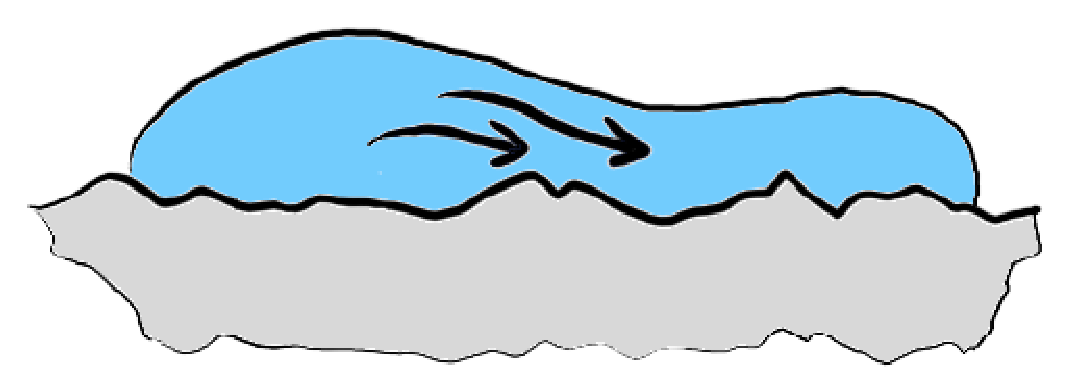
\includegraphics[width=0.30\textwidth]{../images/Curtis1997-layer-shallow-water}
  }
  \par
  \subfloat[pigment-deposition layer]{
    \label{fig:3-schichten-modell-pigment}
    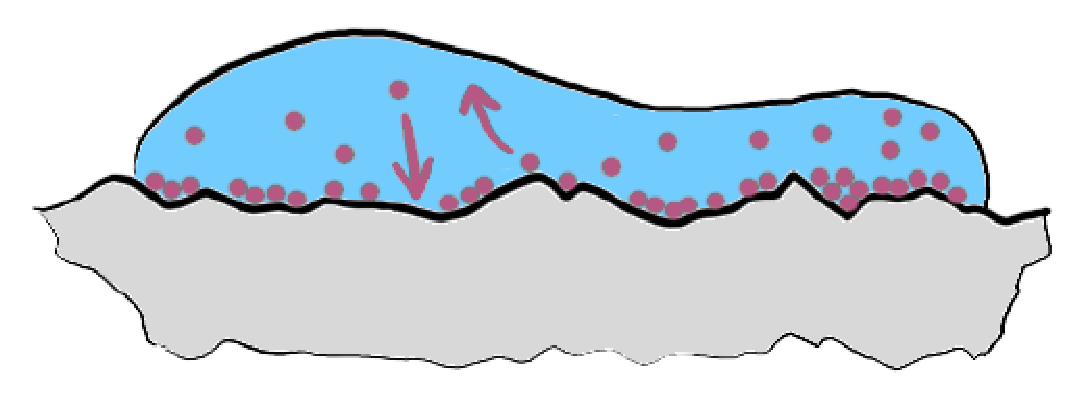
\includegraphics[width=0.30\textwidth]{../images/Curtis1997-layer-pigment-deposition}
  }
  \par
  \subfloat[capillary layer]{
    \label{fig:3-schichten-modell-capillary}
    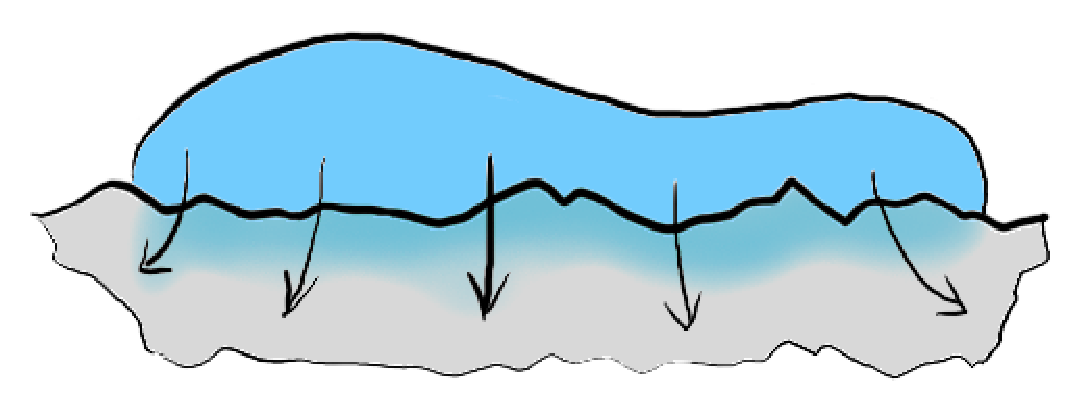
\includegraphics[width=0.30\textwidth]{../images/Curtis1997-layer-capillary}
  }
  \caption{3-Schichten-Modell für die Flüssigkeitssimulation. Quelle: \cite{Curtis1997}.}
  \label{fig:3-schichten-modell}
\end{figure}

Die einzelnen Schichten haben dabei von oben nach unten die folgenden Bedeutungen
und Aufgaben:

\begin{itemize}
  \item Innerhalb des \textsl{shallow-water layer} (dt.\ Flachwasserschicht, 
  Abb.\ \ref{fig:3-schichten-modell-shallow}) können das Wasser und 
  Farbpigmente über die Papieroberfläche transportiert werden.
  \item Auf dem \textsl{pigment-deposition layer} (dt.\ 
  Pigmentablagerungsschicht, Abb.\ \ref{fig:3-schichten-modell-pigment}) 
  können Pigmente abgelagert, bzw.\ von hier auch erneut weiter transportiert 
  werden.
  \item Im \textsl{capillary layer} (dt.\ Kapillarschicht, Abb.\ 
  \ref{fig:3-schichten-modell-capillary}) diffundiert das in das Papier 
  absorbierte Wasser und kann sich somit ausbreiten.
\end{itemize}

\subsubsection{Hauptschleife}
In Listing \ref{lst:mainloop} ist die Hauptschleife der Simulation in 
Pseudocode aufgeführt. Folgende Werte werden der Simulation als Anfangsdaten
übergeben: 

\begin{itemize}
  \item $M$, die sog.\ \textsl{wet-area mask}, die markiert, an welchen Stellen
  das Papier nass ($1$) bzw.\ trocken ist ($0$).
  \item $u$ und $v$, die Geschwindigkeit des Wassers in $x$- bzw.\ $y$-Richtung.
  \item $p$, der Wasserdruck.
  \item $g^k$, die Pigmentkonzentration.
  \item $d^k$, die abgesetzten Pigmente im \textsl{pigment-deposition layer}.
  \item $s$, die Wassersättigung des Papiers.
\end{itemize}

\begin{lstlisting}[caption={Simulationshauptschleife}, label={lst:mainloop}, %
emph={MoveWater, MovePigment, TransferPigment, SimulateCapillaryFlow}, %
emphstyle=]
function MainLoop($M$, $u$, $v$, $p$, $g^1$, ..., $g^n$, $d^1$, ..., $d^n$, $s$):
	for each time step do: (*\label{line:time-step}*)
		MoveWater($M,$ $u$, $v$, $p$)
		MovePigment($M$, $u$, $v$, $g^1$, ..., $g^n$)
		TransferPigment($g^1$, ..., $g^n$, $d^1$, ..., $d^n$)
		SimulateCapillaryFlow($M$, $s$)
	end for
end function
\end{lstlisting}

Wie das Listing zeigt, iteriert die Simulation über eine definierte Anzahl von 
Zeitschritten (Zeile \ref{line:time-step}), führt Wasser- und Pigmentbewegungen 
aus, transferiert Pigmente zwischen den verschiedenen Schichten, haftet diese 
an das Papier an und lässt Wasser durch den \textsl{capillary layer} 
diffundieren.

\subsubsection{Simulationsschritte}
\paragraph{Wasserbewegung} 
Die Bewegungen des Wassers werden im \textsl{shallow-water layer} durchgeführt. 
Einige der Bedingungen für das Verhalten des Wassers lauten dabei:

\begin{enumerate}
  \item Der Wasserfluss muss begrenzt werden durch die \textsl{wet-area mask}.
  \item Wasserüberschuss in einer Region sollte ein Abfließen des Überschusses in
  benachbarte Regionen verursachen.
  \item Lokale Änderungen (z.\,B.\ das Hinzufügen von Wasser an einer Stelle) 
  sollten Auswirkungen auf die komplette Simulation haben.
\end{enumerate}

Listing \ref{lst:watermovement} zeigt die grobe Vorgehensweise bei der 
Simulation der Wasserbewegungen.

\begin{lstlisting}[caption={Wasserbewegung}, label={lst:watermovement}, %
emph={MoveWater, UpdateVelocities, RelaxDivergence, FlowOutward}, %
emphstyle=]
function MoveWater(M, u, v, p):
	UpdateVelocities(M, u, v, p)
	RelaxDivergence(M, u, v, p)
	FlowOutward(M, p)
end function
\end{lstlisting}

Auf die einzelnen Untermethoden soll hier nicht weiter eingegangen, sondern 
deren Funktion nur kurz umrissen werden. \textsl{UpdateVelocities()} ist für
die Aktualisierung der Wassergeschwindigkeiten $u$ und $v$ zuständig.
\textsl{RelaxDivergence()} dient dazu, die Abweichungen des
Geschwindigkeitsfelds zu entspannen. Mittels \textsl{FlowOutward()} wird
schließlich der \textsl{edge darkening}-Effekt simuliert, indem in jedem 
Schritt eine proportional zur Entfernung zum Rand steigende Wassermenge aus den 
Zellen entfernt wird.

\paragraph{Pigmentbewegung}
Pigmente bewegen sich innerhalb der Flachwasserschicht gemäß dem zuvor
berechneten Geschwindigkeitsfeld $u, v$ für das Wasser. Pigmente werden
entsprechend der Flüssigkeitsabflussrate aus einer Zelle in die Nachbarzellen
bewegt. Nachfolgend ist der Pseudocode für die Simulation der Pigmentbewegungen
angegeben. 

\begin{lstlisting}[caption={Pigmentbewegung}, label={lst:pigmentmovement}, %
morekeywords={forall}]
function MovePigment(M, u, v, $g^1$, ..., $g^n$):
	$\Delta t$ = $1/\lceil \max_{i,j}\{|u|, |v|\} \rceil$

	for each pigment k do
		for t = 0 to 1 by $\Delta t$ do
			$g'$ = $g$ = $g^k$

			forall cells ($i$, $j$) do
				$g'_{i+1,j}$ = $g'_{i+1,j}$ + $\max(0, u_{i+0.5,j} g_{i,j})$
				$g'_{i-1,j}$ = $g'_{i-1,j}$ + $\max(0, -u_{i-0.5,j} g_{i,j})$
				$g'_{i,j+1}$ = $g'_{i,j+1}$ + $\max(0, v_{i,j+0.5} g_{i,j})$
				$g'_{i,j-1}$ = $g'_{i,j-1}$ + $\max(0, -v_{i,j-0.5} g_{i,j})$
				$g'_{i,j}$ = $g'_{i,j}$ - $\max(0, u_{i+0.5,j} g_{i,j})$ + $\max(0, -u_{i-0.5,j} g_{i,j})$ + $\max(0, v_{i,j+0.5} g_{i,j})$ + $\max(0, -v_{i,j-0.5} g_{i,j})$
			end for
			$g^k$ = $g'$
		end for
	end for
end function
\end{lstlisting}

\paragraph{Pigmentabsorption und -desorption}
In jedem Simulationsschritt werden Pigmente zu einem gewissen Grad von der 
Pigmentablagerungsschicht absorbiert und auch wieder zurück in die Flüssigkeit 
resorbiert. Mittels der Parameter \textsl{density} (Dichte) und 
\textsl{staining power} (Verschmutzungsfähigkeit) lässt sich festlegen, in 
welchem Maße jedes Pigment ab- bzw.\ resorbiert wird. Weiterhin bestimmt der 
Parameter \textsl{granulation} (Körnung), wie die Papierhöhe $h$ die Ab- und 
Resorption beeinflusst.

Für den Pseudocode dieses Simulationsschritts sei auf den entsprechenden 
Abschnitt der Arbeit von \cite{Curtis1997} verwiesen.

\paragraph{Backrun-Effekt}
Die sog.\ \textsl{Backruns} entstehen, wenn eine Wasserlache sich langsam über
eine trocknende, aber noch feuchte Region ausbreitet. In feuchten Regionen
verteilt sich Flüssigkeit nicht mehr in der Flachwasserschicht, sondern über die
Kapillareffekte in der entsprechenden Kapillarschicht.
Zur Simulation dieses Effekts wird Wasser aus der Flachwasserschicht absorbiert
und diffundiert durch die Kapillarschicht. Jede Zelle überträgt dabei solange
Wasser an die Nachbarzellen, bis diese bis zur Kapazität $c$ gesättigt sind.
Liegt diese Sättigung nun über einem Schwellwert, so wird die \textsl{wet-area
mask} entsprechend erweitert - auf diese Weise kann sich eine Wasserlache durch
die Kapillarvorgänge ausbreiten.

Wie zuvor verweisen wir für den Pseudocode auf die Arbeit von \cite{Curtis1997}.

\subsubsection{Rendering der Wasserfarbenlayer}
Nach Berechnung der einzelnen Wasserfarbenlayer werden diese mithilfe des 
Kubelka-Munk-Farbmodells (KM-Farbmodell) zusammengefügt. Dieses Farbmodell 
erlaubt eine realistischere, aber dementsprechend aufwändigere Darstellung von 
Farbeffekten als z.\,B.\ das RGB-Farbmodell. Es werden dabei für jeden 
Farbkanal des RGB-Farbraums zwei Koeffizienten berechnet:

\begin{enumerate}
  \item Der Absorptionskoeffizient $K$ bestimmt den Anteil der absorbierten 
  Energie.
  \item Der Streuungskoeffzient $S$ bestimmt den Anteil der zurückgestreuten 
  Energie.
\end{enumerate}

Im Gegensatz zur typischen Anwendung der KM-Theorie werden diese Koeffizienten 
nicht experimentell bestimmt, sondern lassen sich vom Benutzer interaktiv 
festlegen. Auf diese Weise lassen sich eine große Anzahl realistisch wirkender 
Farben erzeugen, wie Abbildung \ref{fig:pigments} beispielhaft zeigt.

\begin{figure}
  \centering
  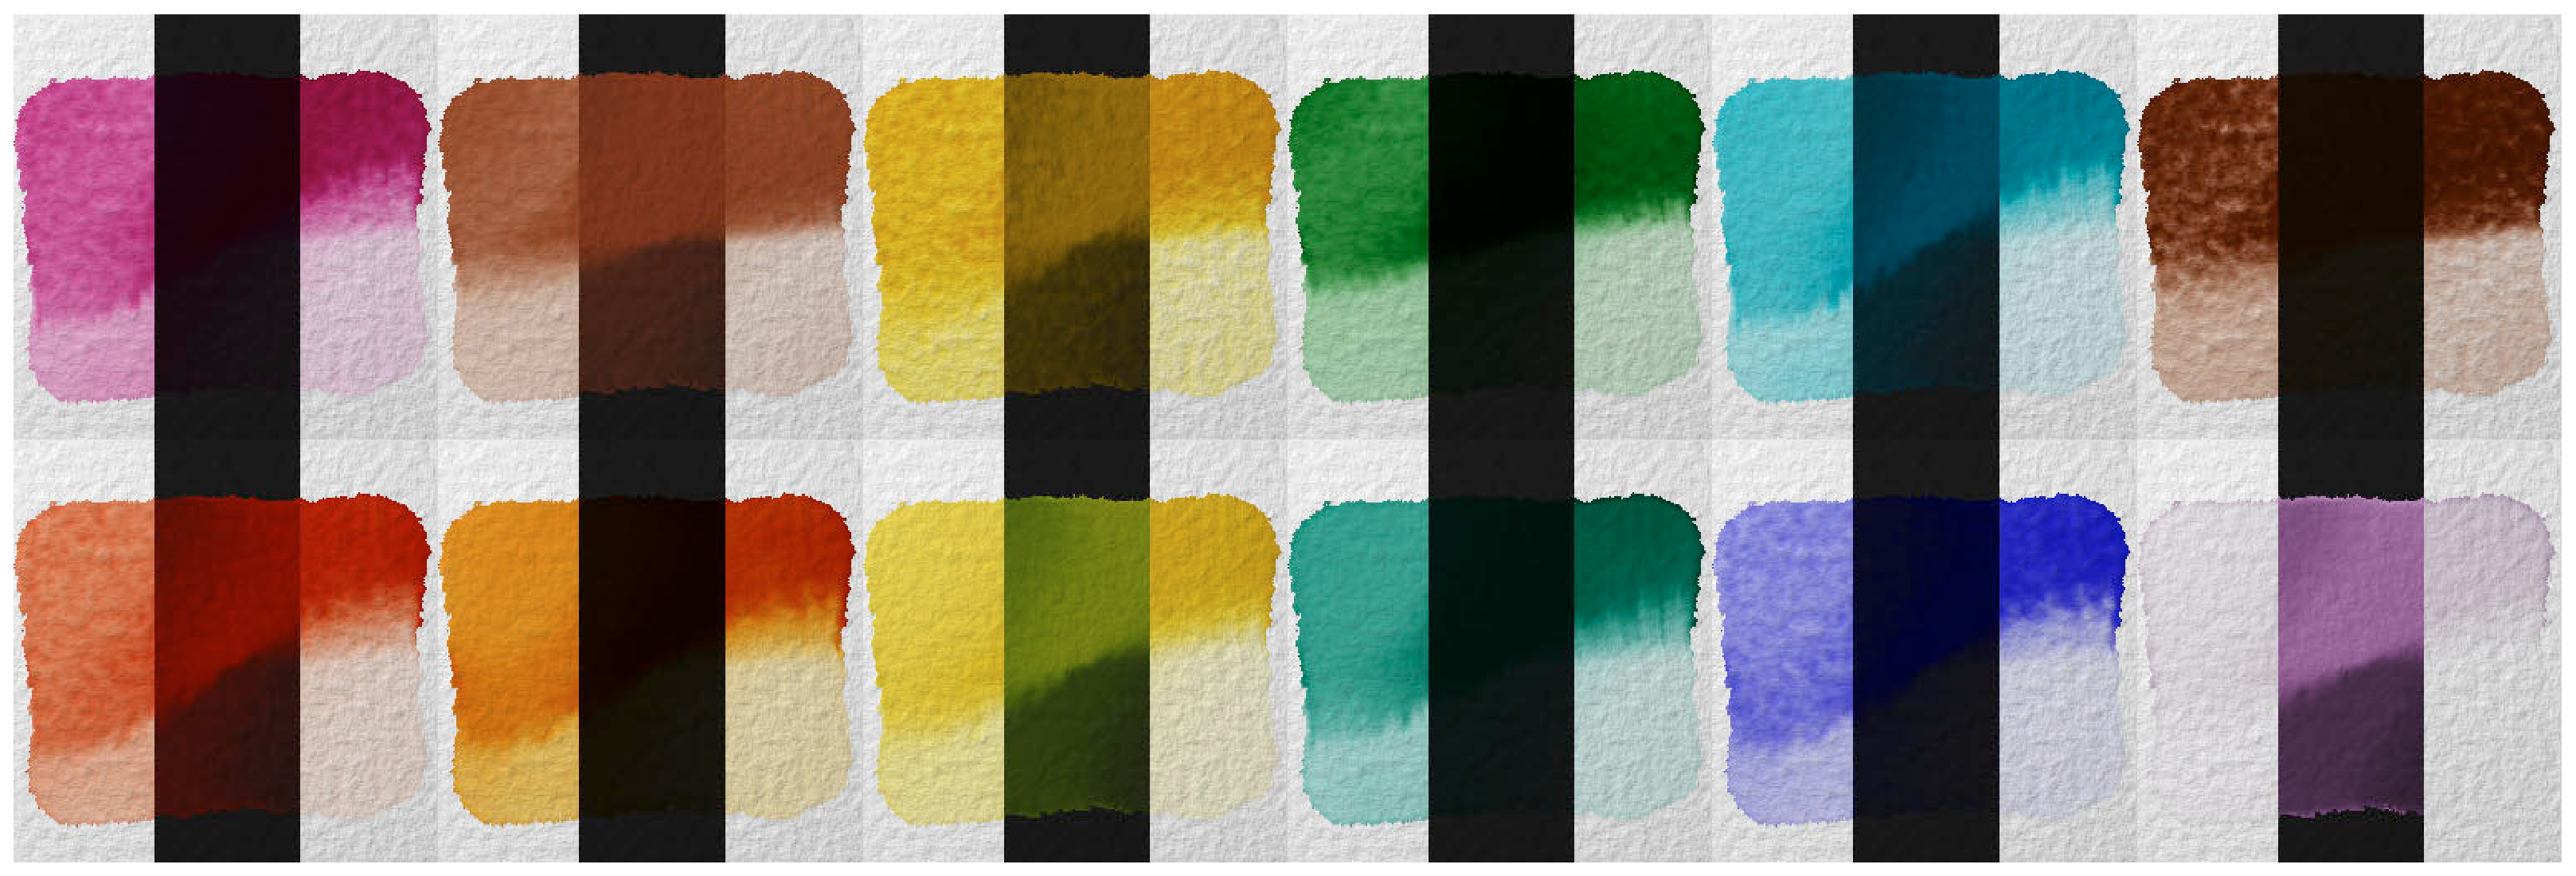
\includegraphics[width=1.00\textwidth]{../images/Curtis1997-pigments}
  \caption{Verschiedene synthetisch erzeugte Pigmente. Quelle: \cite{Curtis1997}.}
  \label{fig:pigments}
\end{figure}

\paragraph{Komposition der Layer}
Nach Ermittlung der Koeffizienten $K$ und $S$ für einen Layer der Dicke $x$ 
kann nun mithilfe des KM-Modells die Reflektion $R$ und der 
Durchlässigkeitsgrad $T$ bestimmt werden:

\begin{eqnarray*}
R &=& \sinh b S x/c \\
T &=& b/c, \qquad c = a \sinh b S x + b \cosh b S x \\
\end{eqnarray*}

Der Wert $x$ errechnet sich aus der Summe der Pigmentkonzentration $g^k$ in der 
Flachwasserschicht und der Konzentration der abgelagerten Pigmente $d^k$ in der 
Pigmentablagerungsschicht. Weiterhin können nun die Werte $R$ und $T$ für zwei 
angrenzende Layer errechnet werden:

\begin{eqnarray*}
  R &=& R_1 + \frac{T^2_1 R_2}{1 - R_1 R_2} \\
  T &=& \frac{T^1 T_2}{1 - R_1 R_2}
\end{eqnarray*}

Diese Berechnung wird für jeden zusätzlichen Layer wiederholt und schließlich
wird die Gesamtreflektion $R$ für die Darstellung des jeweiligen Pixels benutzt.

\subsection{Anwendungen}
Mithilfe des vorgestellten Simulationsverfahrens lassen sich eine Reihe von
Anwendungen realisieren.
Da ist zunächst das \textbf{interaktive Malen} zu erwähnen. Dem Anwender wird
ermöglicht, den "`Startzustand"' der Simulation interaktiv zu malen. Dabei
erstellt er beliebig viele Wasserfarbenlayer, die jeweils Unterlayer für die
Pigmente, das Wasser und die \textsl{wet-area mask} besitzen. Allen Layern
gemein ist ein Referenzbild sowie eine Papiertextur. Außerdem lassen sich
jeweils die physikalischen Eigenschaften der einzelnen Layer sowie die Anzahl
der Simulationsschritte festlegen.
Da die Simulation wie gezeigt doch recht komplex ist, kann diese nicht in
Echtzeit ablaufen. In Kapitel \ref{sec:echtzeit-wasserfarben} stellen wir einen
weiteren Ansatz vor, der Wasserfarbenanimationen von 3D-Szenen in Echtzeit 
erlaubt.

Eine weitere Anwendung ist die sog.\ \textbf{Watercolorization}, bei der ein 
bestehendes Farbbild in eine Wasserfarben-Illustration transformiert wird. Dazu 
wird zunächst eine Farbtrennung durchgeführt, bei der ermittelt wird, in 
welchem Layer welche Pigmentfarbe zu platzieren ist. Anschließend werden beim 
Malen jedes Layers Wasser- oder Pigmentpinselstriche hinzugefügt, um dem 
Ausgangsbild möglichst nah zu kommen. Abbildung \ref{fig:watercolorization} 
zeigt beispielhaft das Ergebnis einer solcher automatischen Kolorierung. Als 
Erweiterung lässt sich dieses Verfahren auch auf 3D-Szenen anwenden.

\begin{figure}
  \centering \subfloat[Ausgangsbild]{
    \label{fig:watercolorization-input}
  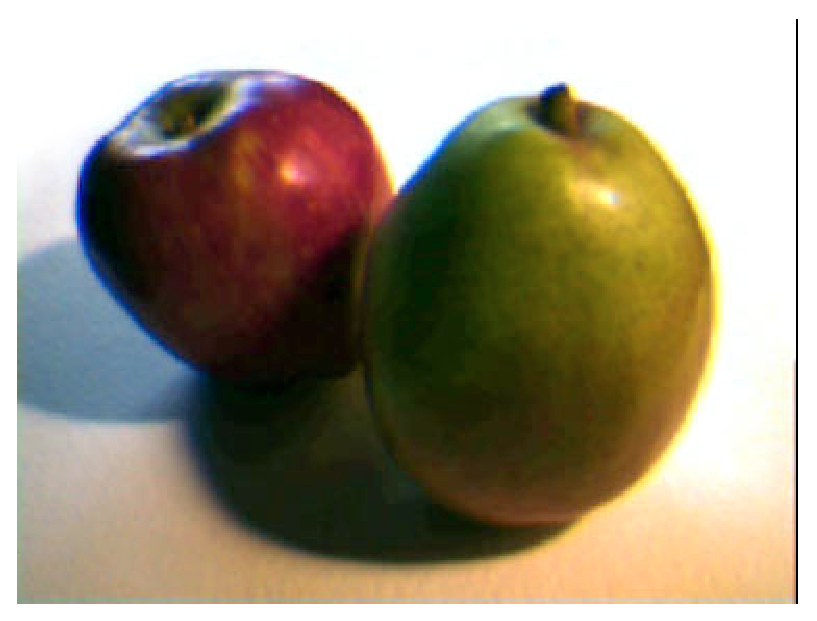
\includegraphics[width=0.40\textwidth]{../images/Curtis1997-watercolorization-input} 
  } \subfloat[Ergebnisbild mit 11 Layern]{
    \label{fig:watercolorization-output}
  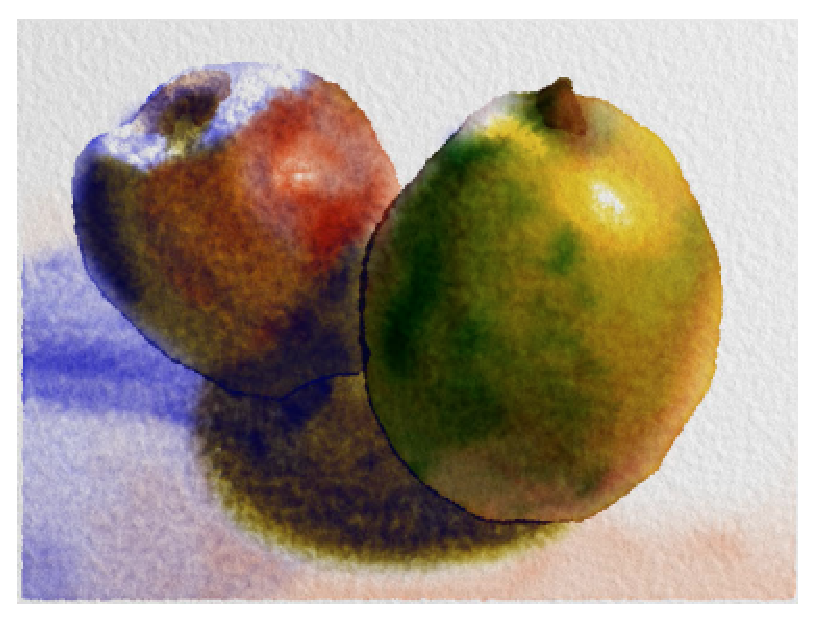
\includegraphics[width=0.40\textwidth]{../images/Curtis1997-watercolorization-output} 
  }
  \caption{Watercolorization, Anzahl der Simulationsschritte: 2750. Quelle: \cite{Curtis1997}.}
  \label{fig:watercolorization}
\end{figure}

\section{Echtzeit-Wasserfarben-Animationen}
\label{sec:echtzeit-wasserfarben}

\subsection{Einleitung}
Im Gegensatz zur zuvor beschriebenen physikalischen Simulation von Wasserfarben 
beschreibt die Arbeit von \cite{Luft2006} Verfahren, mit denen möglichst 
naturgetreue Animationen in Wasserfarbenoptik von 3D-Szenen in 
\textsl{Echtzeit} erstellt werden können. Wie bereits gesehen, erfordert die 
realistische Simulation einen hohen Aufwand, weshalb man sich hier für einen 
Mittelweg zwischen möglichst überzeugender Darstellung und hoher 
Geschwindigkeit der Animation entschieden hat. Es werden die wichtigsten 
Effekte der Wasserfarbenmalerei imitiert und außerdem Licht- und 
Schatteneffekte erzeugt.

\subsection{Abstraktion und Vereinfachung}
Der erste Schritt des Verfahrens beinhaltet die Erstellung einer Anzahl 
abstrakter Wasserfarbenlayern, die alle mehr oder weniger einen gleichförmigen 
Inhalt bzw.\ Farbe haben. In Abbildung \ref{fig:tree-original} sind dies 
beispielsweise die Blätter auf der einen und die Äste auf der anderen Seite. 
Die Ausgangs-3D-Szene wird anhand eindeutiger Identifikatoren segmentiert, das 
Ergebnis (s.\ Abbildung \ref{fig:tree-segmentation}) sind die sog.\ 
\textsl{intensity images} $\rho : \mathbf{N}^2 \to \mathbf{R}$, wobei $\rho(x, 
y) \in [0,1]$. Anschließend wird mithilfe eines Tiefpassfilters (Gauss-Filter) 
der gewünschte Abstraktionsgrad erzielt; es entstehen abstrakte weiche Formen. 
Außerdem erhält jeder Layer eine benutzerdefinierte Farbe $c_{rgb}$ sowie 
Transparenz $c_a$.

\begin{figure}
  \centering
  \subfloat[Photorealistisches Originalmodell]{
    \label{fig:tree-original}
    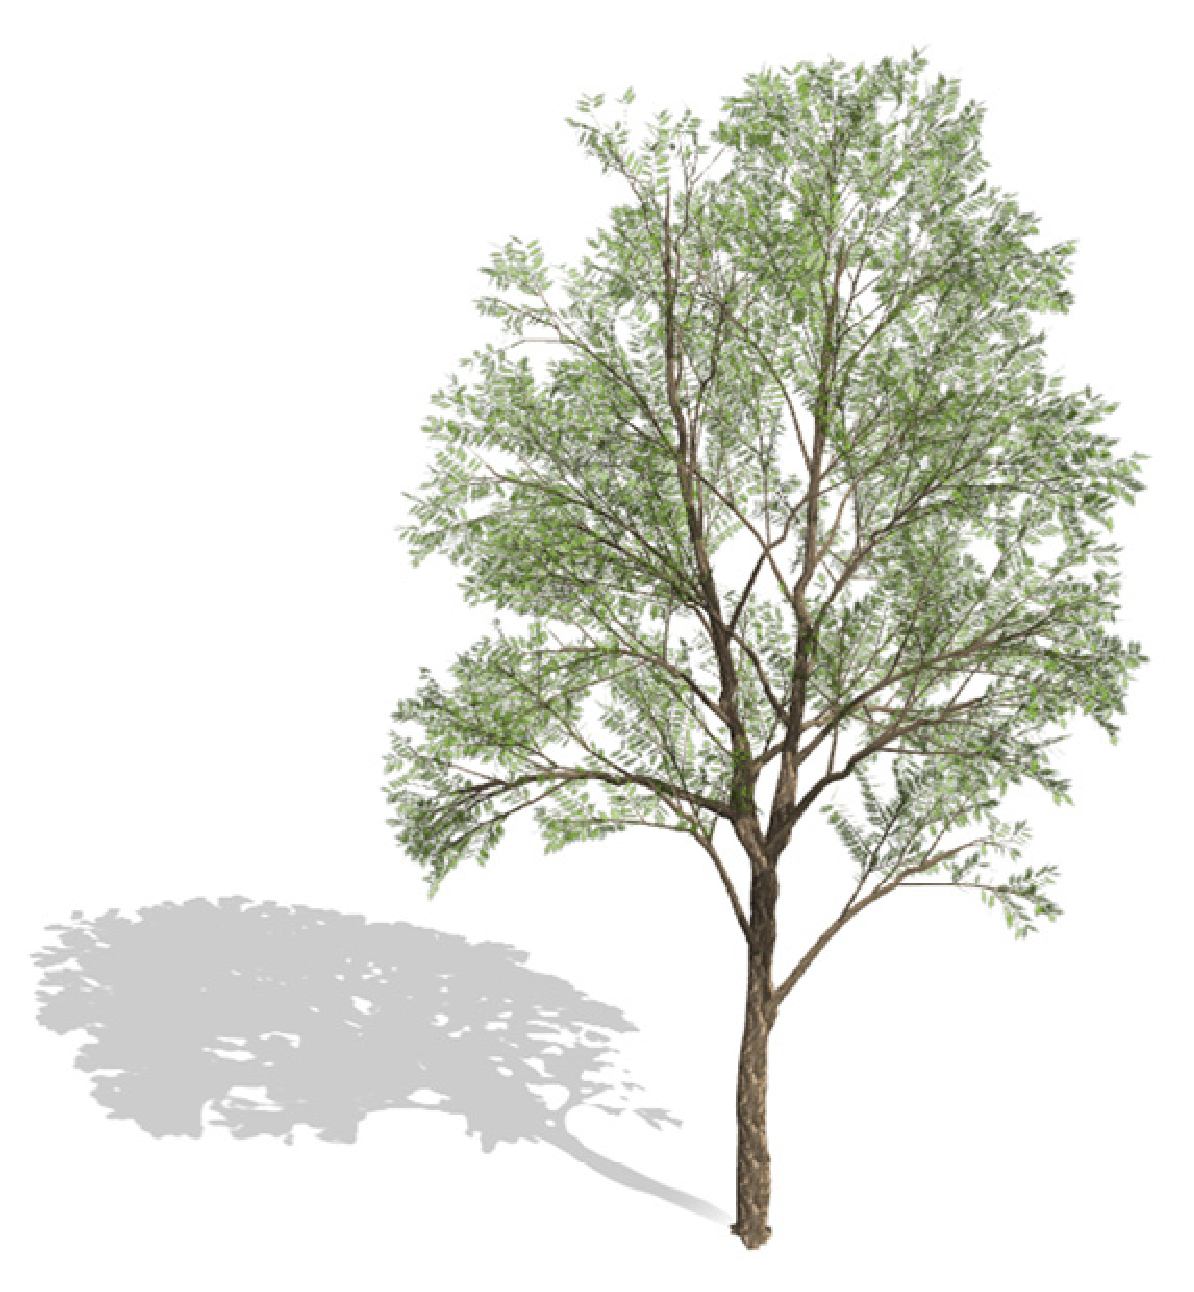
\includegraphics[height=6cm]{../images/Luft2006-tree-original}
  }
  \qquad
  \subfloat[Ergebnis nach der Segmentierung]{
    \label{fig:tree-segmentation}
    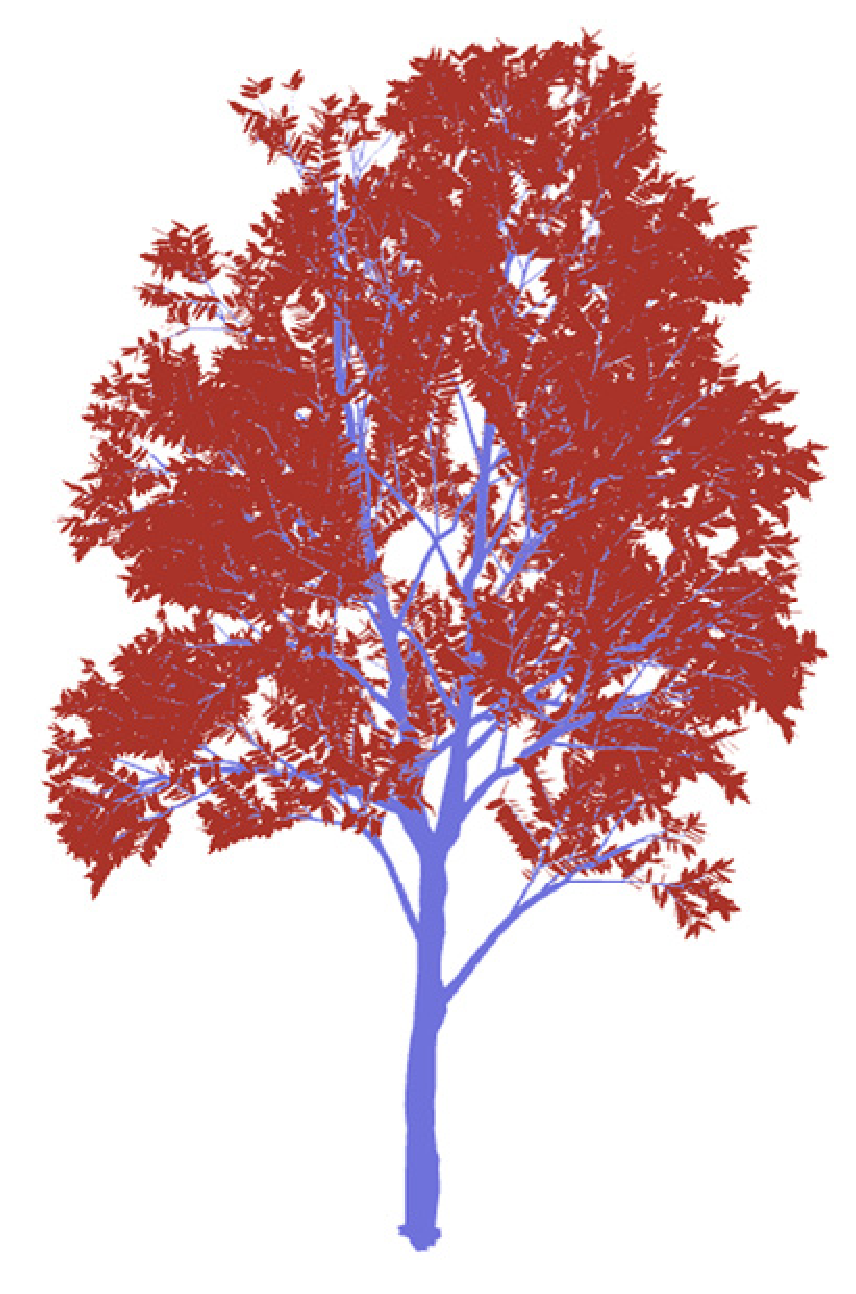
\includegraphics[height=6cm]{../images/Luft2006-tree-segmentation}
  }
  \caption{Abstraktion und Vereinfachung. Quelle: \cite{Luft2006}.}
  \label{fig:original-segmentation}
\end{figure}

\subsection{Formextraktion und Fließmuster}
Die Form eines Wasserfarbenlayers ergibt sich direkt aus den Intensitätswerten 
des entsprechenden \textsl{intensity image} $\rho(x, y)$. Zur Erzeugung einer 
hartkantigen Form des Wasserfarbenlayers wird eine \textsl{step}-Funktion 
angewandt und eine initiale Transparenz berechnet:

\[
\lambda_a(x,y) = c_a \cdot step(\kappa_\rho, \rho(x,y))
\]

Mittels des Parameters $\kappa_\rho$ lässt sich die Ausdehnung des 
Wasserfarbenlayers beeinflussen. Zur Erzeugung der Fließmuster wird die 
\textsl{step}-Funktion durch eine andere Variante ersetzt, bei welcher über 
einen zusätzlichen Parameter die Weichheit der Kanten bestimmt wird - auf diese 
Weise lassen sich das \textsl{wet-on-dry}- und \textsl{wet-on-wet}-painting 
imitieren.

\subsection{Edge darkening}
Dieser bereits beschriebene Effekt wird durch Anwendung des Gauss-Filters
ermöglicht, welcher einen weichen Intensitätsübergang an den Kanten der Layers
erzeugt. Um den Effekt naturgetreu zu imitieren, muss zusätzlich der Rand
verdunkelt dargestellt werden. Dazu wird der Alpha-Kanal $\lambda_a(x,y)$ mittels
der Intensitätswerte angepasst:

\[
\lambda_a(x,y) = \lambda_a(x,y) \cdot (1 + \kappa_\omega \cdot (1 - \rho(x,y)))
\]

Über den Parameter $\kappa_\omega$ kann der Anwender also die Stärke der
Kantenabdunklung festlegen, ein Beispiel nach Durchführung zeigt Abbildung
\ref{fig:tree-edge-darkening}.

\begin{figure}
  \centering
  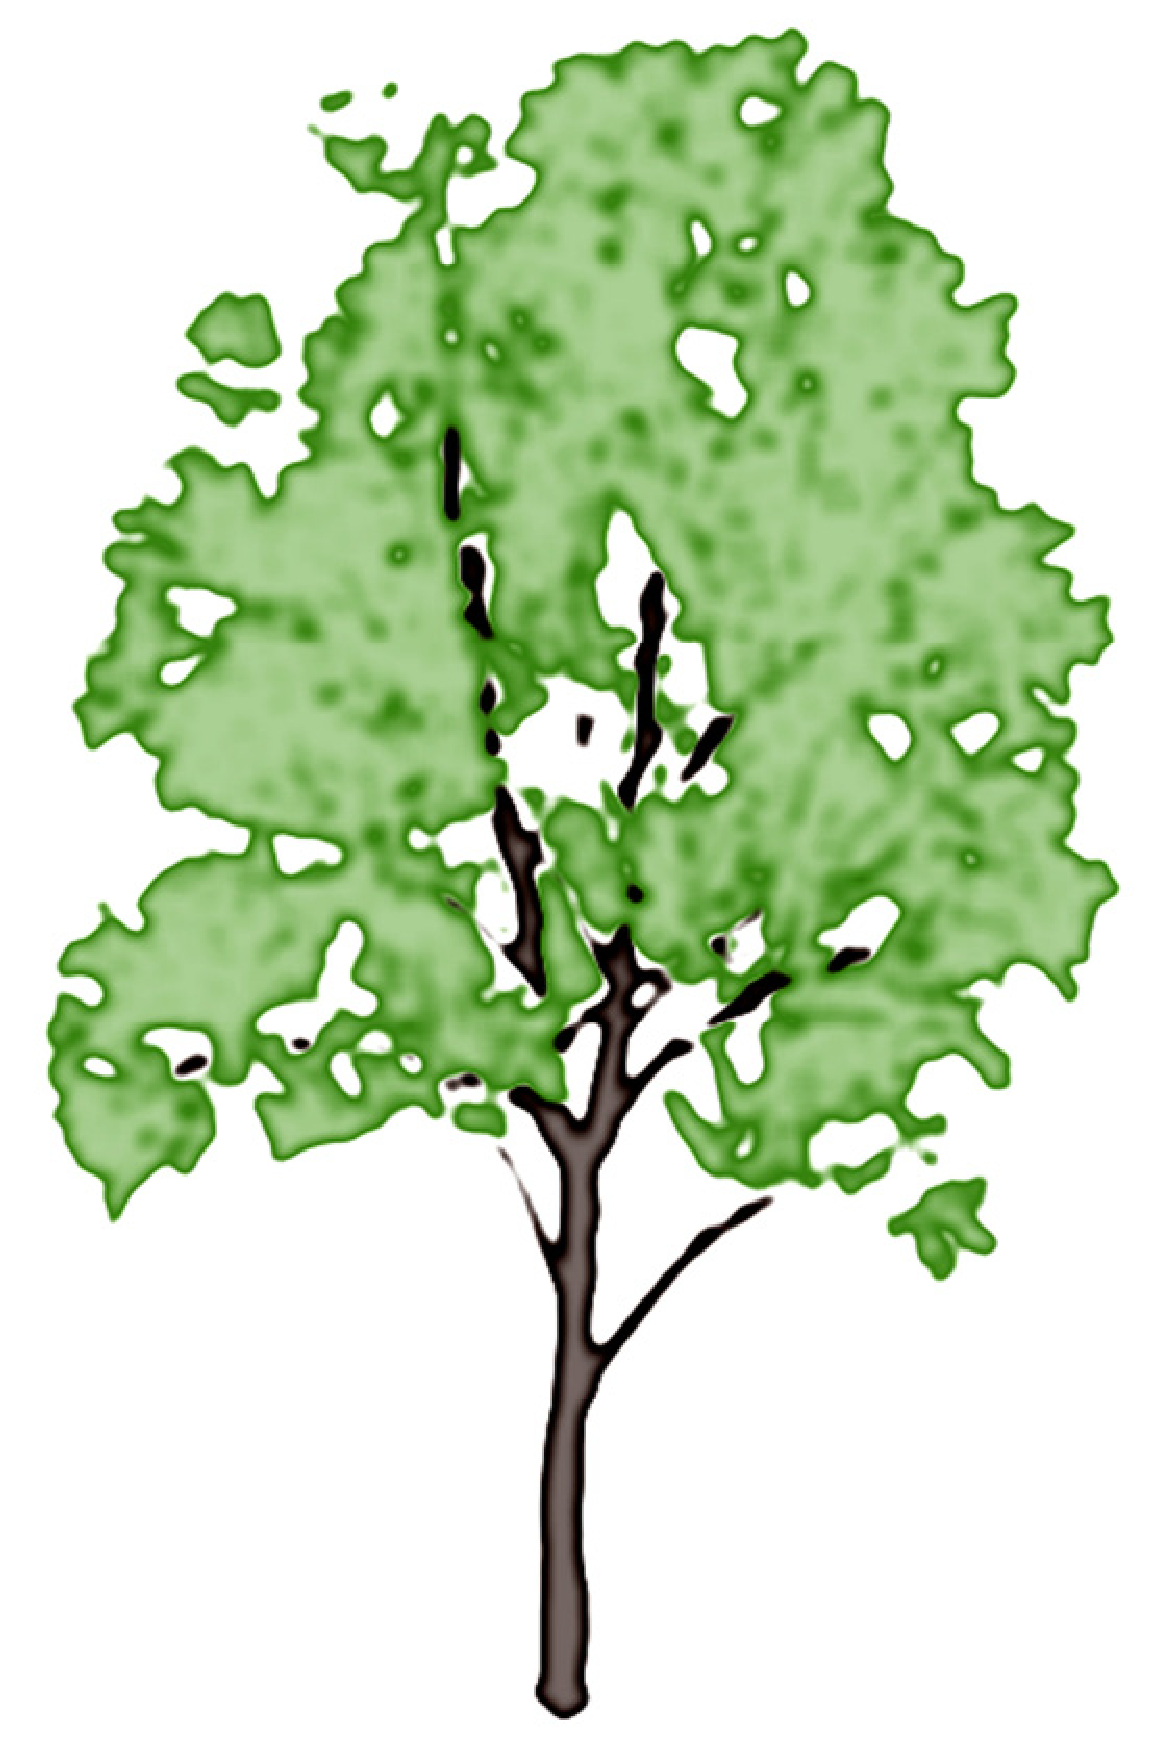
\includegraphics[height=6cm]{../images/Luft2006-tree-edge-darkening}
  \caption{Edge darkening mit $\kappa_\omega = 0.8$. Quelle: \cite{Luft2006}.}
  \label{fig:tree-edge-darkening}
\end{figure}

\subsection{Komposition der Wasserfarben-Layern}
Nach der Erstellung der einzelnen Layer werden evtl.\ zusätzliche Schichten für
Farb- und Schatteneffekte erstellt und aus allen Layern schließlich das
Ergebnisbild zusammengesetzt.

\subsubsection{Licht und Schatten}
Die bereits beschriebene Methode zur Segmentierung der 3D-Szenen ignoriert
all diejenigen Oberflächendetails, die auf Licht und Schatten zurückzuführen
sind. Daher werden die im Modell evtl.\ verfügbaren Beleuchtungsinformationen
zur nachträglichen Anpassung der einzelnen Layer oder Erzeugung neuer verwendet.

Für die Erzeugung der \textbf{Beleuchtungseffekte} wird das 
Phong-Beleuchtungsmodell \cite{Phong1975} benutzt. In diesem Modell wird die 
Reflextion von Licht als Kombination aus ambienter, ideal diffuser und ideal 
spiegelnder Reflexion betrachtet. In diesem Falle wird der ambiente Term als 
konstant und bereits durch die initiale Farbe der Layer gegeben angenommen. Die 
verbleibenden zwei Komponenten werden aus Optimierungsgründen zunächst auf das 
Intervall $[0,1]$ normiert und anschließend auf zwei getrennte \textsl{lighting 
maps} gerendert:

\[
L_d, L_s : \mathbb{N}^2 \to \mathbb{R}
\]

Mithilfe dieser zusätzlichen Layer werden dann alle Wasserfarbenlayer
manipuliert:

\begin{itemize}
  \item Der spiegelnde Term entspricht einer Reflexion von Licht und erzeugt
  somit einen hervorgehobenen Bereich. Objekte, welche aus einem spiegelnden
  Material bestehen, müssen also im \textsl{intensity image} mithilfe der
  entsprechenden \textsl{lighting map} vor Erstellung des Wasserfarbenlayers 
  ausmaskiert werden: 
  \[
  \rho(x,y) = \rho(x,y) \cdot (1- step(\kappa_s, L_s(x,y)))
  \]
  \item Der diffuse Term wird analog dazu benutzt, um neue Layer zu erstellen,
  die dann als Maske für die \textsl{intensity images} benutzt werden. Weiterhin
  werden über diesen Term alle existierenden Wasserfarbenlayer in ihrer Farbe
  angepasst, um das entsprechende diffuse Umgebungslicht zu simulieren.
\end{itemize}

Um zusätzlich \textbf{Schatteneffekte} in die Szene zu integrieren, wird ein
zusätzlicher Layer erstellt, welcher nur die schattierten Regionen beinhaltet.
Zur Berechnung dieses Layers wird ein Standard-Algorithmus zur Berechnung von
Schatten verwendet. Die zuvor beschriebenen Effekte werden auf diesen
zusätzlichen Layer ebenfalls angewandt, inklusive des diffusen Umgebungslichts.

\subsubsection{Komposition}
Im Gegensatz zum Ansatz von \cite{Curtis1997} wird hier zur abschließenden 
Komposition (s.\ Abbildung \ref{fig:tree-result}) der einzelnen Layer nicht das 
Kubelka-Munk-Modell eingesetzt, sondern die Standard-Blending-Funktionen für 
transparente Objekte (Alpha-Blending). Die endgültige Farbe $C_{rgb}$ eines 
Pixels bestimmt sich mithilfe der Farbe $C_{rgb}$ und Transparenz $C_a$ des 
aktuellen Layers sowie der Hintergrundfarbe $B_{rgb}$:

\[
R_{rgb} = C_a \cdot C_{rgb} + (1 - C_a) \cdot B_{rgb}
\]

\begin{figure}
  \centering
  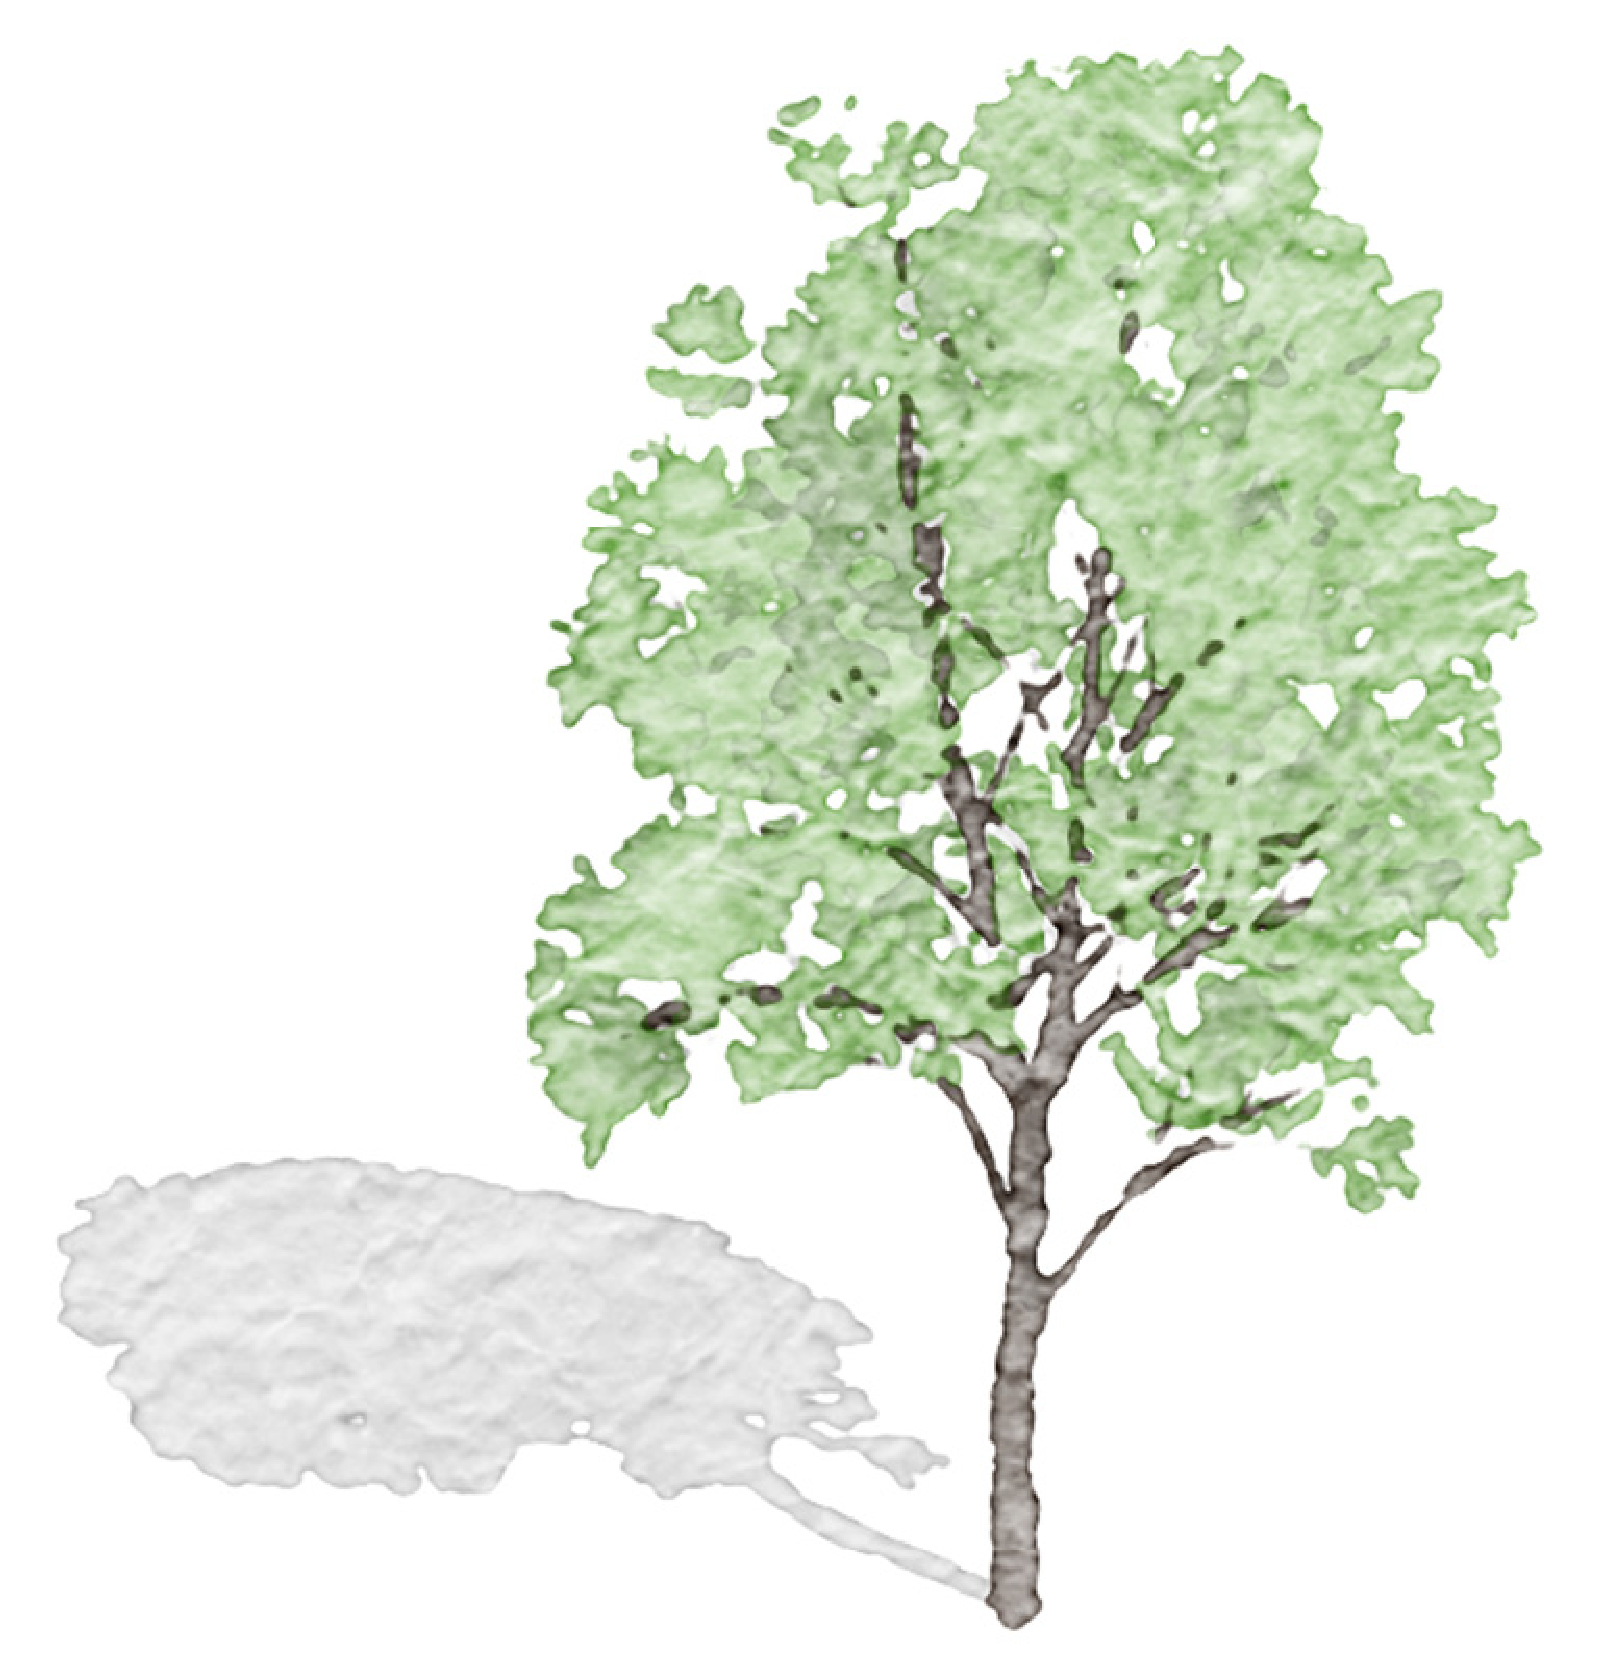
\includegraphics[height=6cm]{../images/Luft2006-tree-result}
  \caption{Endergebnis mit Schattenwurf. Quelle: \cite{Luft2006}.}
  \label{fig:tree-result}
\end{figure}

\subsection{Ergebnisse}
Abschließend stellen wir hier einige weiter Beispielbilder der Echtzeitanimation
vor. Alle Bilder wurden dabei mit einer Auflösung von 720 x 720 Pixel gerendert.

\begin{figure}
  \centering
  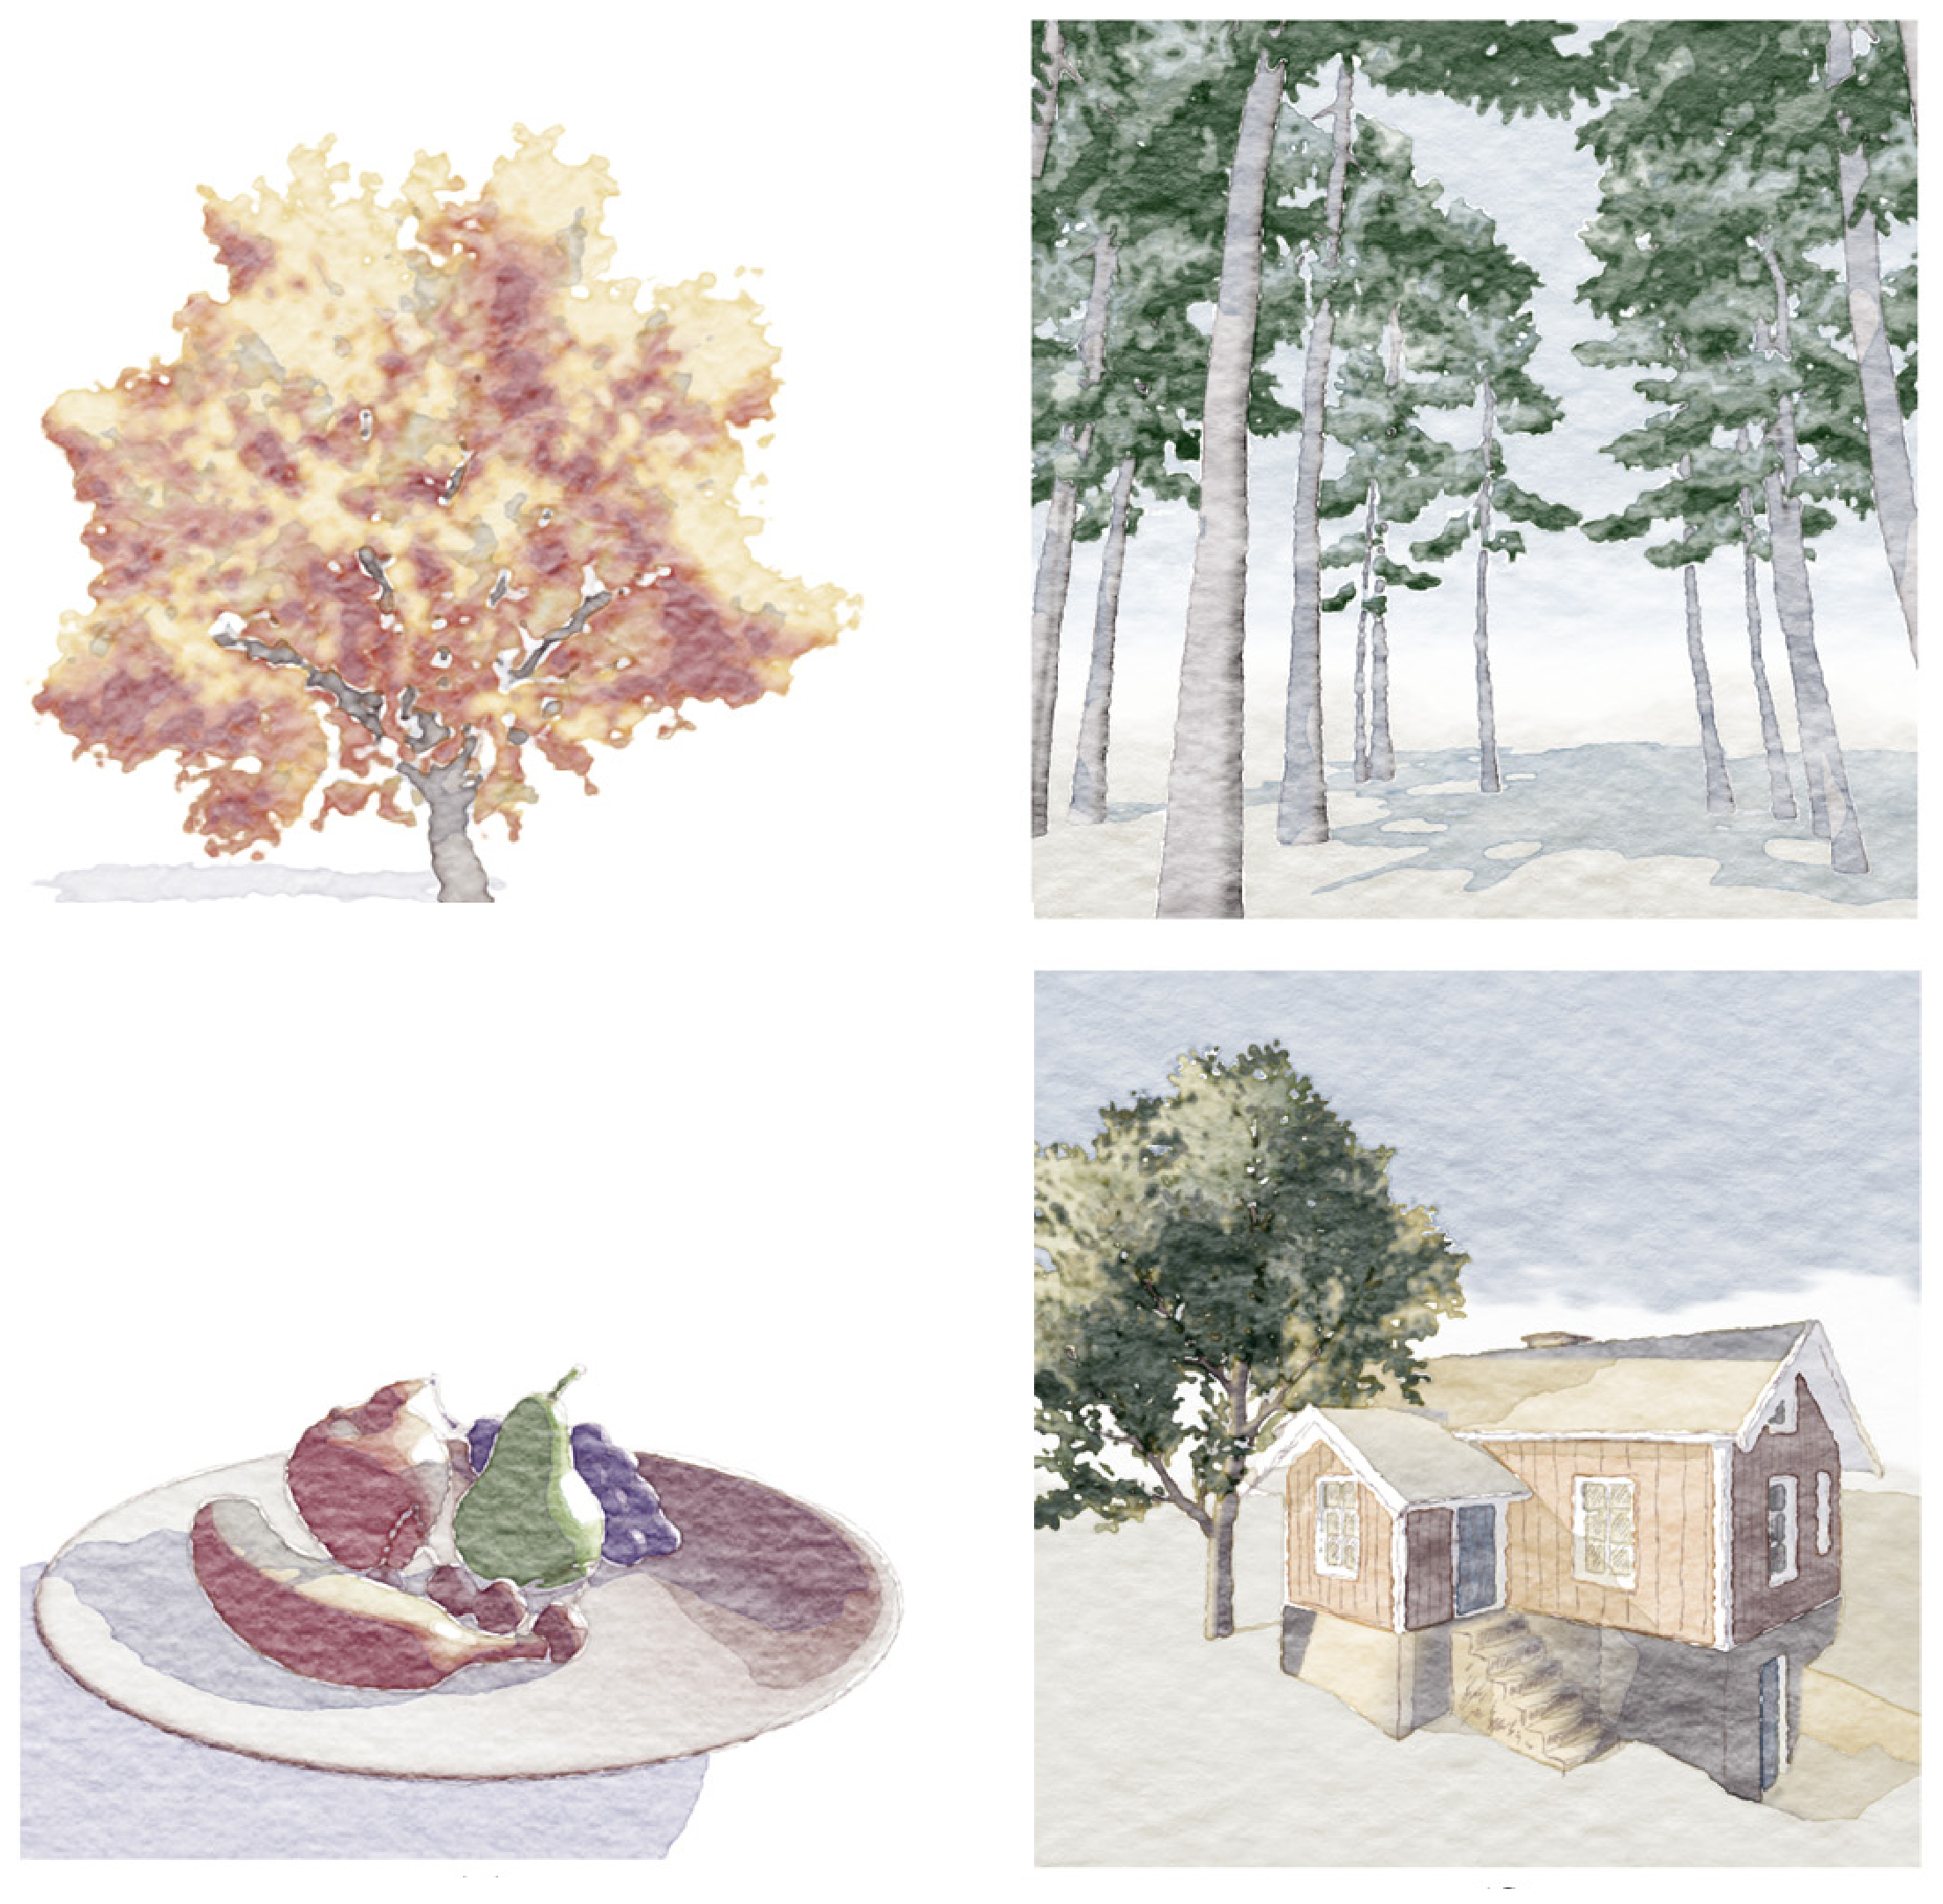
\includegraphics[width=0.8\textwidth]{../images/Luft2006-examples}
  \caption{Beispielbilder aus der Echtzeitanimation. Quelle: \cite{Luft2006}.}
  \label{fig:wcolor-results}
\end{figure}

%%% Inkludieren Kapitel 6
\chapter{Fazit}
Zusammenfassend ist zu sagen, dass das \textbf{Non-Photorealistic-Rendering} eine 
Alternative zum Photorealismus bietet und die Informationsvermittlung 
vielseitig in Form von verschiedenartigen Bildern unterstützt. Auf Grund der 
vielen verschiedenen Techniken und Möglichkeiten, die NPR bietet, ist ein 
Einsatz in einer Vielzahl von unterschiedlichen Anwendungsbereichen möglich und 
eine optimale Anpassung an bestimmte Aufgaben ist gewährleistet.


%%%
%%% Anhaenge: Glossar, Bibliographie...
%%%

%\cleardoublepage % oder \clearpage
%\phantomsection 

%\appendix
%\pdfbookmark[-1]{\appendixname}{\appendixname} 

%%% Bibliographie-Stil
% abbrvdin, alphadin, plaindin, unsrtdin
\bibliographystyle{alphadin}

%%% Anstatt 'Literatur' -> 'Quellen'
\renewcommand{\bibname}{Quellen}

%%% Bibliographie ausgeben
\bibliography{../Literatur}

%%% Glossar ausgeben
%\printgloss{Glossar}

\end{document}
%%% END OF FILE